\documentclass[11pt]{article}
\usepackage{graphicx}
\usepackage[export]{adjustbox}
\usepackage{multicol}
\marginparwidth0.0in
\evensidemargin 0.0in
\oddsidemargin 0.0in
\textwidth 6.67in
\setlength{\topmargin}{0.0in}
\setlength{\textheight}{9.2in}
\pagestyle{myheadings}
\begin{document}
\pagenumbering{arabic}
\pagebreak 
\setcounter{page}{1}
\vskip 0.1in 

\begin{center}ASTR 1030 - FALL 2017 - EXAM \#7 - WALLIN
\vskip 0.1in 

\center{\LARGE VERSION 1} 
\end{center}
Instructions (Read carefully): 
\begin{enumerate}
\item ABSOLUTELY NO TALKING OR PHONE USE! 
\item {\bf Do not open the exam until you are directed to do so by your instructor!}
\item Write your name, M\#, and your clicker Device ID on the cover sheet below. 
\item Read and sign the Honor Code Certification below.
\item Use your M\# for your ID on the clicker.
\item This is test version 1
\item Read the questions carefully. 
\item Mark all your answers on the paper exam and THEN enter them in your clicker after you have completed the exam with a pen/pencil.
\item When you have completed the exam, turn in the exam to the LA at the front of the room and have your picture ID ready for inspection.
\item GOOD LUCK!!! 
\end{enumerate}
\hrulefill 
\vskip 0.1in 

\begin{itemize} \item Print your name :
\vskip 0.25in 


\item M \# :
\vskip 0.25in 

\item Clicker Device ID : 
\end{itemize} 
\vskip 0.5in 

{\bf Honor Code Certification}
\bigskip

I certify that I have abided by the MTSU honor code in taking this examination. The work
on this exam is my own. I have received no assistance from other persons in completing
this exam. 
\bigskip

Signature:


\pagebreak 

\begin{enumerate}
\setlength{\itemsep}{1pt} 
\setlength{\parskip}{0pt} 
\setlength{\parsep}{0pt}
\setlength{\multicolsep}{1pt} 

\begin{minipage}{\textwidth}
\begin{minipage}{\textwidth}
\item Latitude and longitude measure:
\begin{enumerate} 
\setlength{\itemsep}{1pt} 
\setlength{\parskip}{0pt} 
\setlength{\parsep}{0pt}
\setlength{\multicolsep}{1pt} 
\item *Position on Earth.
\item Position of objects in the sky measured from the perspective of a particular observer.
\item Positions of objects in the sky which are the same for all observers.
\item Positions on the Moon.
\end{enumerate} 
Objective = 1.1
Index = 76
Source = testbank
Scramble = Y
Type = MC
\end{minipage}
\end{minipage}
\vskip 0.20in

\begin{minipage}{\textwidth}
\begin{minipage}{\textwidth}
\item Latitude and longitude measure:
\begin{enumerate} 
\setlength{\itemsep}{1pt} 
\setlength{\parskip}{0pt} 
\setlength{\parsep}{0pt}
\setlength{\multicolsep}{1pt} 
\item *Positions on Earth
\item Positions in the sky as seen locally
\item Positions in the sky which are the same for all observers
\end{enumerate} 
Objective = 1.1
Index = 170
Source = clicker
Scramble = N
Type = MC
\end{minipage}
\end{minipage}
\vskip 0.20in

\begin{minipage}{\textwidth}
\begin{minipage}{\textwidth}
\item How many constellations cover surface of the Celestial Sphere?
\begin{multicols}{3}
\begin{enumerate} 
\setlength{\itemsep}{1pt} 
\setlength{\parskip}{0pt} 
\setlength{\parsep}{0pt}
\setlength{\multicolsep}{1pt} 
\item 45
\item *88
\item 120
\item No one knows.
\end{enumerate} 
\vfill 
\end{multicols}

Objective = 1.2
Index = 108
Source = testbank
Scramble = N
Type = MC
\end{minipage}
\end{minipage}
\vskip 0.20in

\begin{minipage}{\textwidth}
\begin{minipage}{\textwidth}
\item The stars in a constellation are physically close to one another.
\begin{multicols}{3}
\begin{enumerate} 
\setlength{\itemsep}{1pt} 
\setlength{\parskip}{0pt} 
\setlength{\parsep}{0pt}
\setlength{\multicolsep}{1pt} 
\item True
\item *False
\end{enumerate} 
\vfill 
\end{multicols}

Objective = 1.2
Index = 115
Source = homework
Scramble = N
Type = TF
\end{minipage}
\end{minipage}
\vskip 0.20in

\begin{minipage}{\textwidth}
\begin{minipage}{\textwidth}
\item The celestial sphere is divided into 88 modern constellations.
\begin{multicols}{3}
\begin{enumerate} 
\setlength{\itemsep}{1pt} 
\setlength{\parskip}{0pt} 
\setlength{\parsep}{0pt}
\setlength{\multicolsep}{1pt} 
\item *True
\item False
\end{enumerate} 
\vfill 
\end{multicols}

Objective = 1.2
Index = 122
Source = homework
Scramble = N
Type = TF
\end{minipage}
\end{minipage}
\vskip 0.20in

\begin{minipage}{\textwidth}
\begin{minipage}{\textwidth}
\item Constellations are close clusters of stars, all at about the same distance from the Sun.
\begin{multicols}{3}
\begin{enumerate} 
\setlength{\itemsep}{1pt} 
\setlength{\parskip}{0pt} 
\setlength{\parsep}{0pt}
\setlength{\multicolsep}{1pt} 
\item True
\item *False
\end{enumerate} 
\vfill 
\end{multicols}

Objective = 1.2
Index = 131
Source = homework
Scramble = N
Type = TF
\end{minipage}
\end{minipage}
\vskip 0.20in

\begin{minipage}{\textwidth}
\begin{minipage}{\textwidth}
\item Altitude and azimuth measure:
\begin{enumerate} 
\setlength{\itemsep}{1pt} 
\setlength{\parskip}{0pt} 
\setlength{\parsep}{0pt}
\setlength{\multicolsep}{1pt} 
\item Position on Earth.
\item *Position of objects in the sky measured from the perspective of a particular observer.
\item Positions of objects in the sky which are the same for all observers.
\item Positions on the Moon.
\end{enumerate} 
Objective = 1.4
Index = 77
Source = testbank
Scramble = Y
Type = MC
\end{minipage}
\end{minipage}
\vskip 0.20in

\begin{minipage}{\textwidth}
\begin{minipage}{\textwidth}
\item Right ascension and declination measure:
\begin{enumerate} 
\setlength{\itemsep}{1pt} 
\setlength{\parskip}{0pt} 
\setlength{\parsep}{0pt}
\setlength{\multicolsep}{1pt} 
\item Position on Earth.
\item Position of objects in the sky measured from the perspective of a particular observer.
\item *Positions of objects in the sky which are the same for all observers.
\item Positions on the Moon.
\end{enumerate} 
Objective = 1.4
Index = 78
Source = testbank
Scramble = Y
Type = MC
\end{minipage}
\end{minipage}
\vskip 0.20in

\begin{minipage}{\textwidth}
\begin{minipage}{\textwidth}
\item The closest terrestrial analog to hours of right ascension is angle of longitude.
\begin{multicols}{3}
\begin{enumerate} 
\setlength{\itemsep}{1pt} 
\setlength{\parskip}{0pt} 
\setlength{\parsep}{0pt}
\setlength{\multicolsep}{1pt} 
\item *True
\item False
\end{enumerate} 
\vfill 
\end{multicols}

Objective = 1.4
Index = 110
Source = homework
Scramble = N
Type = TF
\end{minipage}
\end{minipage}
\vskip 0.20in

\begin{minipage}{\textwidth}
\begin{minipage}{\textwidth}
\item From the horizon to the observer's zenith is an angle of...
\begin{multicols}{3}
\begin{enumerate} 
\setlength{\itemsep}{1pt} 
\setlength{\parskip}{0pt} 
\setlength{\parsep}{0pt}
\setlength{\multicolsep}{1pt} 
\item Azimuth
\item Declination
\item Right Ascension
\item Altitude
\item *Latitude
\end{enumerate} 
\vfill 
\end{multicols}

Objective = 1.4
Index = 118
Source = homework
Scramble = Y
Type = TF
\end{minipage}
\end{minipage}
\vskip 0.20in

\begin{minipage}{\textwidth}
\begin{minipage}{\textwidth}
\item Latitude and right ascension are coordinate systems used to find objects on the celestial sphere.
\begin{multicols}{3}
\begin{enumerate} 
\setlength{\itemsep}{1pt} 
\setlength{\parskip}{0pt} 
\setlength{\parsep}{0pt}
\setlength{\multicolsep}{1pt} 
\item True
\item *False
\end{enumerate} 
\vfill 
\end{multicols}

Objective = 1.4
Index = 129
Source = homework
Scramble = N
Type = TF
\end{minipage}
\end{minipage}
\vskip 0.20in

\begin{minipage}{\textwidth}
\begin{minipage}{\textwidth}
\item In the sky, declination is measured in degrees north or south of the celestial equator.
\begin{multicols}{3}
\begin{enumerate} 
\setlength{\itemsep}{1pt} 
\setlength{\parskip}{0pt} 
\setlength{\parsep}{0pt}
\setlength{\multicolsep}{1pt} 
\item *True
\item False
\end{enumerate} 
\vfill 
\end{multicols}

Objective = 1.4
Index = 130
Source = homework
Scramble = N
Type = TF
\end{minipage}
\end{minipage}
\vskip 0.20in

\begin{minipage}{\textwidth}
\begin{minipage}{\textwidth}
\item Altitude and azimuth measure:
\begin{enumerate} 
\setlength{\itemsep}{1pt} 
\setlength{\parskip}{0pt} 
\setlength{\parsep}{0pt}
\setlength{\multicolsep}{1pt} 
\item Positions on Earth
\item *Positions in the sky as seen locally
\item Positions in the sky which are the same for all observers
\end{enumerate} 
Objective = 1.4
Index = 171
Source = clicker
Scramble = N
Type = MC
\end{minipage}
\end{minipage}
\vskip 0.20in

\begin{minipage}{\textwidth}
\begin{minipage}{\textwidth}
\item Right ascension and declination measure:
\begin{enumerate} 
\setlength{\itemsep}{1pt} 
\setlength{\parskip}{0pt} 
\setlength{\parsep}{0pt}
\setlength{\multicolsep}{1pt} 
\item Positions on Earth
\item Positions in the sky as seen locally
\item *Positions in the sky which are the same for all observers
\end{enumerate} 
Objective = 1.4
Index = 172
Source = clicker
Scramble = N
Type = MC
\end{minipage}
\end{minipage}
\vskip 0.20in

\begin{minipage}{\textwidth}
\begin{minipage}{\textwidth}
\item A star's altitude is:
\begin{enumerate} 
\setlength{\itemsep}{1pt} 
\setlength{\parskip}{0pt} 
\setlength{\parsep}{0pt}
\setlength{\multicolsep}{1pt} 
\item The distance it is above the Earth's surface.
\item The distance between the star and the Sun.
\item The angle between the star and the Celestial equator.
\item The angle compass heading of a star measured by an observer.
\item *The angle between the star and the horizon of the observer.
\end{enumerate} 
Objective = 1.4
Index = 206
Source = testbank
Scramble = Y
Type = MC
\end{minipage}
\end{minipage}
\vskip 0.20in

\begin{minipage}{\textwidth}
\begin{minipage}{\textwidth}
\item A star's azimuth is:
\begin{enumerate} 
\setlength{\itemsep}{1pt} 
\setlength{\parskip}{0pt} 
\setlength{\parsep}{0pt}
\setlength{\multicolsep}{1pt} 
\item The distance it is above the Earth's surface.
\item The distance between the star and the Sun.
\item The angle bewteen the star and the Celestial equator.
\item *The angle compass heading of a star measured by an observer.
\item The angle between the star and the horizon of the observer.
\end{enumerate} 
Objective = 1.4
Index = 207
Source = testbank
Scramble = Y
Type = MC
\end{minipage}
\end{minipage}
\vskip 0.20in

\begin{minipage}{\textwidth}
\begin{minipage}{\textwidth}
\item A star's declination is:
\begin{enumerate} 
\setlength{\itemsep}{1pt} 
\setlength{\parskip}{0pt} 
\setlength{\parsep}{0pt}
\setlength{\multicolsep}{1pt} 
\item The distance it is above the Earth's surface.
\item The distance between the star and the Sun.
\item *The angle bewteen the star and the Celestial equator.
\item The angle compass heading of a star measured by an observer.
\item The angle between the star and the horizon of the observer.
\end{enumerate} 
Objective = 1.4
Index = 208
Source = testbank
Scramble = Y
Type = MC
\end{minipage}
\end{minipage}
\vskip 0.20in

\begin{minipage}{\textwidth}
\begin{minipage}{\textwidth}
\item Late one night, you call up a friend who lives 200 mile directly North of {\bf Murfreesboro}.   You both look North and see the star Polaris.  Your friend will observe that Polaris is:
\begin{enumerate} 
\setlength{\itemsep}{1pt} 
\setlength{\parskip}{0pt} 
\setlength{\parsep}{0pt}
\setlength{\multicolsep}{1pt} 
\item shifted directly down toward the horizon compared to Murfreesboro.
\item *shifted directly up from the horizon compared to  Murfreesboro.
\item shifted up and to the right compared to Murfreesboro.
\item shifted down and to the left  compared to Murfreesboro.
\item shifted down and to the right compared to Murfreesboro.
\end{enumerate} 
Objective = 2.2
Index = 9
Source = testbank
Scramble = Y
Type = MC
\end{minipage}
\end{minipage}
\vskip 0.20in

\begin{minipage}{\textwidth}
\begin{minipage}{\textwidth}
\item Late one night, you call up a friend who lives 200 mile directly South of {\bf Murfreesboro}.   You both look North and see the star Polaris.  Your friend will observe that Polaris is:
\begin{enumerate} 
\setlength{\itemsep}{1pt} 
\setlength{\parskip}{0pt} 
\setlength{\parsep}{0pt}
\setlength{\multicolsep}{1pt} 
\item *shifted directly down toward the horizon compared to Murfreesboro.
\item shifted directly up from the horizon compared to  Murfreesboro.
\item shifted up and to the right compared to Murfreesboro.
\item shifted down and to the left  compared to Murfreesboro.
\item shifted down and to the right compared to Murfreesboro.
\end{enumerate} 
Objective = 2.2
Index = 209
Source = testbank
Scramble = Y
Type = MC
\end{minipage}
\end{minipage}
\vskip 0.20in

\begin{minipage}{\textwidth}
\begin{minipage}{\textwidth}
\item As viewed from above the North Pole, which direction does the Earth rotate?
\begin{multicols}{3}
\begin{enumerate} 
\setlength{\itemsep}{1pt} 
\setlength{\parskip}{0pt} 
\setlength{\parsep}{0pt}
\setlength{\multicolsep}{1pt} 
\item Clockwise
\item *Counter-clockwise
\item Left
\item Right
\end{enumerate} 
\vfill 
\end{multicols}

Objective = 2.3
Index = 173
Source = clicker
Scramble = N
Type = MC
\end{minipage}
\end{minipage}
\vskip 0.20in

\begin{minipage}{\textwidth}
\begin{minipage}{\textwidth}
\item We now know that daily motion in the sky is caused by the \underline{\hspace{0.5in}}.
\begin{multicols}{2}
\begin{enumerate} 
\setlength{\itemsep}{1pt} 
\setlength{\parskip}{0pt} 
\setlength{\parsep}{0pt}
\setlength{\multicolsep}{1pt} 
\item *Rotation of the Earth.
\item Revolution of the Earth around the Sun.
\item Revolution of the Sun around the Earth.
\item Precession of the equinoxes.
\end{enumerate} 
\vfill 
\end{multicols}

Objective = 2.4
Index = 84
Source = testbank
Scramble = Y
Type = MC
\end{minipage}
\end{minipage}
\vskip 0.20in

\begin{minipage}{\textwidth}
\begin{minipage}{\textwidth}
\item For this question, assume that {\bf Figure 3} shows the position of the Sun in {\bf Murfreesboro} about an hour before Sunset.   Which letter is closest to where the Sun will be in one hour?
\begin{multicols}{3}
\begin{enumerate} 
\setlength{\itemsep}{1pt} 
\setlength{\parskip}{0pt} 
\setlength{\parsep}{0pt}
\setlength{\multicolsep}{1pt} 
\item Position A
\item Position B
\item Position C
\item Position D
\item *Position E
\end{enumerate} 
\vfill 
\end{multicols}

Objective = 2.4
Index = 91
Source = testbank
Scramble = N
Type = MC
\end{minipage}
\end{minipage}
\vskip 0.20in

\begin{minipage}{\textwidth}
\begin{minipage}{\textwidth}
\item {\bf For this question only,} assume that {\bf Figure 3} shows the position of the Sun in {\bf Murfreesboro} about an hour before Sunset.   Which letter is closest to where the Sun was one hour ago?
\begin{multicols}{3}
\begin{enumerate} 
\setlength{\itemsep}{1pt} 
\setlength{\parskip}{0pt} 
\setlength{\parsep}{0pt}
\setlength{\multicolsep}{1pt} 
\item *Position A
\item Position B
\item Position C
\item Position D
\item Position E
\end{enumerate} 
\vfill 
\end{multicols}

Objective = 2.4
Index = 92
Source = testbank
Scramble = N
Type = MC
\end{minipage}
\end{minipage}
\vskip 0.20in

\begin{minipage}{\textwidth}
\begin{minipage}{\textwidth}
\item Where will the Sun be in two hours?
\begin{multicols}{3}
\begin{enumerate} 
\setlength{\itemsep}{1pt} 
\setlength{\parskip}{0pt} 
\setlength{\parsep}{0pt}
\setlength{\multicolsep}{1pt} 
\item A.
\item B
\item C
\item D
\item *E
\end{enumerate} 
\vfill 
\end{multicols}

Objective = 2.4
Index = 174
Source = clicker
Scramble = N
Type = MC
\end{minipage}
\end{minipage}
\vskip 0.20in

\begin{minipage}{\textwidth}
\begin{minipage}{\textwidth}
\item Where will the Sun be at 7 am on December 28?
\begin{multicols}{3}
\begin{enumerate} 
\setlength{\itemsep}{1pt} 
\setlength{\parskip}{0pt} 
\setlength{\parsep}{0pt}
\setlength{\multicolsep}{1pt} 
\item A
\item B
\item *C
\item D
\item E
\end{enumerate} 
\vfill 
\end{multicols}

Objective = 2.4
Index = 175
Source = clicker
Scramble = N
Type = MC
\end{minipage}
\end{minipage}
\vskip 0.20in

\begin{minipage}{\textwidth}
\begin{minipage}{\textwidth}
\item Where will the Sun be at 9am on December 28?
\begin{multicols}{3}
\begin{enumerate} 
\setlength{\itemsep}{1pt} 
\setlength{\parskip}{0pt} 
\setlength{\parsep}{0pt}
\setlength{\multicolsep}{1pt} 
\item A
\item B
\item C
\item *D
\item E
\end{enumerate} 
\vfill 
\end{multicols}

Objective = 2.4
Index = 176
Source = clicker
Scramble = N
Type = MC
\end{minipage}
\end{minipage}
\vskip 0.20in

\begin{minipage}{\textwidth}
\begin{minipage}{\textwidth}
\item Which direction will the Sun appear to move in the next hour?
\begin{multicols}{2}
\begin{enumerate} 
\setlength{\itemsep}{1pt} 
\setlength{\parskip}{0pt} 
\setlength{\parsep}{0pt}
\setlength{\multicolsep}{1pt} 
\item Up and to the left
\item *Up and to the right
\item Down and to the left
\item Down and to the right
\end{enumerate} 
\vfill 
\end{multicols}

Objective = 2.4
Index = 179
Source = clicker
Scramble = N
Type = MC
\end{minipage}
\end{minipage}
\vskip 0.20in

\begin{minipage}{\textwidth}
\begin{minipage}{\textwidth}
\item Late one night, you call up a friend who lives 200 miles directly West of {\bf Murfreesboro}.   You both go outside to look at the Moon.   You see the first quarter Moon is setting over the Western horizon.   Your friend will see that the Moon is:
\begin{enumerate} 
\setlength{\itemsep}{1pt} 
\setlength{\parskip}{0pt} 
\setlength{\parsep}{0pt}
\setlength{\multicolsep}{1pt} 
\item shifted  up and to the right compared to Murfreesboro.
\item shifted down and to the left  compared to Murfreesboro.
\item *shifted up and to the left compared to Murfreesboro.
\item not visible and below the horizon.
\item being eclipsed by the Earth.
\end{enumerate} 
Objective = 2.5
Index = 10
Source = testbank
Scramble = Y
Type = MC
\end{minipage}
\end{minipage}
\vskip 0.20in

\begin{minipage}{\textwidth}
\begin{minipage}{\textwidth}
\item {\bf For this question only,} assume that {\bf Figure 3} shows the position of the Sun in {\bf Murfreesboro} about an hour after Sunrise.   Which letter is closest to where the Sun was one hour ago?
\begin{multicols}{3}
\begin{enumerate} 
\setlength{\itemsep}{1pt} 
\setlength{\parskip}{0pt} 
\setlength{\parsep}{0pt}
\setlength{\multicolsep}{1pt} 
\item Position A
\item Position B
\item *Position C
\item Position D
\item Position E
\end{enumerate} 
\vfill 
\end{multicols}

Objective = 2.5
Index = 95
Source = testbank
Scramble = N
Type = MC
\end{minipage}
\end{minipage}
\vskip 0.20in

\begin{minipage}{\textwidth}
\begin{minipage}{\textwidth}
\item Circumpolar stars
\begin{enumerate} 
\setlength{\itemsep}{1pt} 
\setlength{\parskip}{0pt} 
\setlength{\parsep}{0pt}
\setlength{\multicolsep}{1pt} 
\item *Always rise in the East.
\item Always set in the West.
\item Never rise or set.
\item Are seen toward the south in Murfreesboro.
\end{enumerate} 
Objective = 2.6
Index = 51
Source = testbank
Scramble = Y
Type = MC
\end{minipage}
\end{minipage}
\vskip 0.20in

\begin{minipage}{\textwidth}
\begin{minipage}{\textwidth}
\item Which star will Ursa Major appear to circle every day?
\begin{multicols}{3}
\begin{enumerate} 
\setlength{\itemsep}{1pt} 
\setlength{\parskip}{0pt} 
\setlength{\parsep}{0pt}
\setlength{\multicolsep}{1pt} 
\item Thuban
\item The Sun
\item *Polaris
\item Mizar/Alcor
\end{enumerate} 
\vfill 
\end{multicols}

Objective = 2.6
Index = 177
Source = clicker
Scramble = N
Type = MC
\end{minipage}
\end{minipage}
\vskip 0.20in

\begin{minipage}{\textwidth}
\begin{minipage}{\textwidth}
\item Which star will the Sun appear to circle around every day?
\begin{multicols}{3}
\begin{enumerate} 
\setlength{\itemsep}{1pt} 
\setlength{\parskip}{0pt} 
\setlength{\parsep}{0pt}
\setlength{\multicolsep}{1pt} 
\item Thuban
\item The Sun
\item *Polaris
\item Mizar/Alcor
\end{enumerate} 
\vfill 
\end{multicols}

Objective = 2.6
Index = 180
Source = clicker
Scramble = N
Type = MC
\end{minipage}
\end{minipage}
\vskip 0.20in

\begin{minipage}{\textwidth}
\begin{minipage}{3.0in}
\item In {\bf Figure 1} at the back of the test, which direction will the stars near letter (d) move if you viewed the sky one hour later.
\begin{multicols}{2}
\begin{enumerate} 
\setlength{\itemsep}{1pt} 
\setlength{\parskip}{0pt} 
\setlength{\parsep}{0pt}
\setlength{\multicolsep}{1pt} 
\item down
\item up
\item *left
\item right
\end{enumerate} 
\vfill 
\end{multicols}

Objective = 3.1
Index = 1
Source = testbank
Scramble = Y
Type = MC
\end{minipage}
\hspace{0.5in}
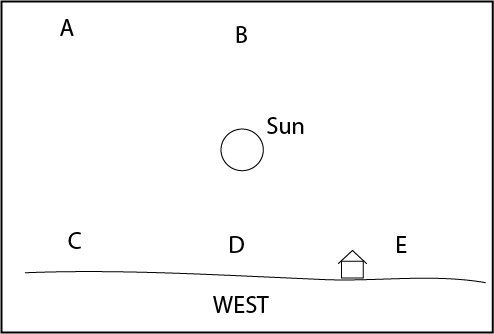
\includegraphics[width=2in,height=1.5in,valign=c]{sunset.png}
\end{minipage}
\vskip 0.20in

\begin{minipage}{\textwidth}
\begin{minipage}{\textwidth}
\item Looking North from {\bf Murfreesboro}, stars appear to rotate counter-clockwise around the star Polaris.
\begin{multicols}{3}
\begin{enumerate} 
\setlength{\itemsep}{1pt} 
\setlength{\parskip}{0pt} 
\setlength{\parsep}{0pt}
\setlength{\multicolsep}{1pt} 
\item *True
\item False
\end{enumerate} 
\vfill 
\end{multicols}

Objective = 3.1
Index = 63
Source = testbank
Scramble = N
Type = MC
\end{minipage}
\end{minipage}
\vskip 0.20in

\begin{minipage}{\textwidth}
\begin{minipage}{\textwidth}
\item In {\bf Figure 1} at the back of the test, which direction will the stars near letter (e) move if you viewed the sky one hour later.
\begin{multicols}{2}
\begin{enumerate} 
\setlength{\itemsep}{1pt} 
\setlength{\parskip}{0pt} 
\setlength{\parsep}{0pt}
\setlength{\multicolsep}{1pt} 
\item down and to the left
\item *down and to the right
\item up and to the left
\item up and to the right
\end{enumerate} 
\vfill 
\end{multicols}

Objective = 3.1
Index = 86
Source = testbank
Scramble = Y
Type = MC
\end{minipage}
\end{minipage}
\vskip 0.20in

\begin{minipage}{\textwidth}
\begin{minipage}{\textwidth}
\item In {\bf Figure 1} at the back of the test, which direction will the stars near letter (A) move if you viewed the sky one hour later.
\begin{multicols}{2}
\begin{enumerate} 
\setlength{\itemsep}{1pt} 
\setlength{\parskip}{0pt} 
\setlength{\parsep}{0pt}
\setlength{\multicolsep}{1pt} 
\item *up and to the left
\item up and to the right
\item down and to the left
\item down and to the right
\end{enumerate} 
\vfill 
\end{multicols}

Objective = 3.1
Index = 98
Source = testbank
Scramble = N
Type = MC
\end{minipage}
\end{minipage}
\vskip 0.20in

\begin{minipage}{\textwidth}
\begin{minipage}{\textwidth}
\item In {\bf Figure 1}, over the next few hours the constellation near the letter {\bf A} will move:
\begin{multicols}{2}
\begin{enumerate} 
\setlength{\itemsep}{1pt} 
\setlength{\parskip}{0pt} 
\setlength{\parsep}{0pt}
\setlength{\multicolsep}{1pt} 
\item down and to the left
\item down and to the right
\item *up and to the left
\item up and to the right
\end{enumerate} 
\vfill 
\end{multicols}

Objective = 3.1
Index = 109
Source = testbank
Scramble = y
Type = MC
\end{minipage}
\end{minipage}
\vskip 0.20in

\begin{minipage}{\textwidth}
\begin{minipage}{\textwidth}
\item Which direction will Ursa Major appear to move in the next hour?
\begin{multicols}{2}
\begin{enumerate} 
\setlength{\itemsep}{1pt} 
\setlength{\parskip}{0pt} 
\setlength{\parsep}{0pt}
\setlength{\multicolsep}{1pt} 
\item Up and to the left
\item Up and to the right
\item Down and to the left
\item *Down and to the right
\end{enumerate} 
\vfill 
\end{multicols}

Objective = 3.1
Index = 178
Source = clicker
Scramble = N
Type = MC
\end{minipage}
\end{minipage}
\vskip 0.20in

\begin{minipage}{\textwidth}
\begin{minipage}{\textwidth}
\item If you are looking East from {\bf Murfreesboro} and the Moon is near the horizon, over the next few hours, the Moon will move:
\begin{multicols}{2}
\begin{enumerate} 
\setlength{\itemsep}{1pt} 
\setlength{\parskip}{0pt} 
\setlength{\parsep}{0pt}
\setlength{\multicolsep}{1pt} 
\item down and to the left
\item down and to the right
\item up and to the left
\item *up and to the right
\end{enumerate} 
\vfill 
\end{multicols}

Objective = 3.2
Index = 7
Source = testbank
Scramble = y
Type = MC
\end{minipage}
\end{minipage}
\vskip 0.20in

\begin{minipage}{\textwidth}
\begin{minipage}{\textwidth}
\item If you are watching the Sun set in {\bf Murfreesboro}, the direction it travels over the Western horizon is
\begin{multicols}{2}
\begin{enumerate} 
\setlength{\itemsep}{1pt} 
\setlength{\parskip}{0pt} 
\setlength{\parsep}{0pt}
\setlength{\multicolsep}{1pt} 
\item down and to the left
\item *down and to the right
\item up and to the left
\item up and to the right
\end{enumerate} 
\vfill 
\end{multicols}

Objective = 3.2
Index = 8
Source = testbank
Scramble = y
Type = MC
\end{minipage}
\end{minipage}
\vskip 0.20in

\begin{minipage}{\textwidth}
\begin{minipage}{\textwidth}
\item If you are on the equator and see the Sun to the East on the Horizon, it will rise
\begin{multicols}{2}
\begin{enumerate} 
\setlength{\itemsep}{1pt} 
\setlength{\parskip}{0pt} 
\setlength{\parsep}{0pt}
\setlength{\multicolsep}{1pt} 
\item *straight up above the horizon.
\item up and to the right.
\item up and to the left.
\item straight down toward the horizon.
\end{enumerate} 
\vfill 
\end{multicols}

Objective = 3.2
Index = 50
Source = testbank
Scramble = Y
Type = MC
\end{minipage}
\end{minipage}
\vskip 0.20in

\begin{minipage}{\textwidth}
\begin{minipage}{\textwidth}
\item For this question, assume that {\bf Figure 3} shows the position of the Sun at the {\bf Equator} about an hour before Sunset.   Which letter is closest to where the Sun will be in one hour?
\begin{multicols}{3}
\begin{enumerate} 
\setlength{\itemsep}{1pt} 
\setlength{\parskip}{0pt} 
\setlength{\parsep}{0pt}
\setlength{\multicolsep}{1pt} 
\item Position A
\item Position B
\item Position C
\item *Position D
\item Position E
\end{enumerate} 
\vfill 
\end{multicols}

Objective = 3.2
Index = 93
Source = testbank
Scramble = N
Type = MC
\end{minipage}
\end{minipage}
\vskip 0.20in

\begin{minipage}{\textwidth}
\begin{minipage}{\textwidth}
\item For this question, assume that {\bf Figure 3} shows the position of the Sun at the {\bf Equator} about an hour before Sunset.   Which letter is closest to where the Sun was one hour ago?
\begin{multicols}{3}
\begin{enumerate} 
\setlength{\itemsep}{1pt} 
\setlength{\parskip}{0pt} 
\setlength{\parsep}{0pt}
\setlength{\multicolsep}{1pt} 
\item Position A
\item *Position B
\item Position C
\item Position D
\item Position E
\end{enumerate} 
\vfill 
\end{multicols}

Objective = 3.2
Index = 94
Source = testbank
Scramble = N
Type = MC
\end{minipage}
\end{minipage}
\vskip 0.20in

\begin{minipage}{\textwidth}
\begin{minipage}{\textwidth}
\item {\bf For this question only,} assume that {\bf Figure 3} shows the position of the Sun at the {\bf Equator} about an hour after Sunrise.   Which letter is closest to where the Sun will be in one hour?
\begin{multicols}{3}
\begin{enumerate} 
\setlength{\itemsep}{1pt} 
\setlength{\parskip}{0pt} 
\setlength{\parsep}{0pt}
\setlength{\multicolsep}{1pt} 
\item Position A
\item *Position B
\item Position C
\item Position D
\item Position E
\end{enumerate} 
\vfill 
\end{multicols}

Objective = 3.2
Index = 96
Source = testbank
Scramble = N
Type = MC
\end{minipage}
\end{minipage}
\vskip 0.20in

\begin{minipage}{\textwidth}
\begin{minipage}{\textwidth}
\item For this question, assume that {\bf Figure 3} shows the position of the Sun at the {\bf Equator} about an hour after Sunrise.   Which letter is closest to where the Sun was \underline{\bf one hour ago}?
\begin{multicols}{3}
\begin{enumerate} 
\setlength{\itemsep}{1pt} 
\setlength{\parskip}{0pt} 
\setlength{\parsep}{0pt}
\setlength{\multicolsep}{1pt} 
\item Position A
\item Position B
\item Position C
\item *Position D
\item Position E
\end{enumerate} 
\vfill 
\end{multicols}

Objective = 3.2
Index = 97
Source = testbank
Scramble = N
Type = MC
\end{minipage}
\end{minipage}
\vskip 0.20in

\begin{minipage}{\textwidth}
\begin{minipage}{\textwidth}
\item The North Celestial Pole is:
\begin{enumerate} 
\setlength{\itemsep}{1pt} 
\setlength{\parskip}{0pt} 
\setlength{\parsep}{0pt}
\setlength{\multicolsep}{1pt} 
\item Just another name for the North Pole.
\item *The location in the sky where you find Polaris.
\item The location directly above the Earth's Equator.
\item One of the places the Sun travels over its yearly journey across the celestial sphere.
\end{enumerate} 
Objective = 3.3
Index = 104
Source = testbank
Scramble = N
Type = MC
\end{minipage}
\end{minipage}
\vskip 0.20in

\begin{minipage}{\textwidth}
\begin{minipage}{\textwidth}
\item The  Celestial Equator is:
\begin{enumerate} 
\setlength{\itemsep}{1pt} 
\setlength{\parskip}{0pt} 
\setlength{\parsep}{0pt}
\setlength{\multicolsep}{1pt} 
\item Just another name for the North Pole.
\item The location in the sky where you find Polaris.
\item *The places in the sky that are  directly above the Earth's Equator.
\item One of the places the Sun travels over its yearly journey across the celestial sphere.
\end{enumerate} 
Objective = 3.3
Index = 107
Source = testbank
Scramble = N
Type = MC
\end{minipage}
\end{minipage}
\vskip 0.20in

\begin{minipage}{\textwidth}
\begin{minipage}{\textwidth}
\item Into how many constellations is the celestial sphere divided?
\begin{multicols}{3}
\begin{enumerate} 
\setlength{\itemsep}{1pt} 
\setlength{\parskip}{0pt} 
\setlength{\parsep}{0pt}
\setlength{\multicolsep}{1pt} 
\item 12
\item 45
\item *88
\item 120
\end{enumerate} 
\vfill 
\end{multicols}

Objective = 3.3
Index = 114
Source = homework
Scramble = N
Type = MC
\end{minipage}
\end{minipage}
\vskip 0.20in

\begin{minipage}{\textwidth}
\begin{minipage}{\textwidth}
\item Which direction are we looking?
\begin{multicols}{3}
\begin{enumerate} 
\setlength{\itemsep}{1pt} 
\setlength{\parskip}{0pt} 
\setlength{\parsep}{0pt}
\setlength{\multicolsep}{1pt} 
\item *North
\item East
\item South
\item West
\end{enumerate} 
\vfill 
\end{multicols}

Objective = 3.4
Index = 181
Source = clicker
Scramble = N
Type = MC
\end{minipage}
\end{minipage}
\vskip 0.20in

\begin{minipage}{\textwidth}
\begin{minipage}{\textwidth}
\item Over a few hours, which direction will the stars move in this region of the sky?
\begin{multicols}{2}
\begin{enumerate} 
\setlength{\itemsep}{1pt} 
\setlength{\parskip}{0pt} 
\setlength{\parsep}{0pt}
\setlength{\multicolsep}{1pt} 
\item Up
\item Down
\item *Clockwise around Polaris
\item Counter-Clockwise around Polaris
\end{enumerate} 
\vfill 
\end{multicols}

Objective = 3.4
Index = 182
Source = clicker
Scramble = N
Type = MC
\end{minipage}
\end{minipage}
\vskip 0.20in

\begin{minipage}{\textwidth}
\begin{minipage}{\textwidth}
\item This picture of stars setting in the West was taken:
\begin{enumerate} 
\setlength{\itemsep}{1pt} 
\setlength{\parskip}{0pt} 
\setlength{\parsep}{0pt}
\setlength{\multicolsep}{1pt} 
\item *At the Equator
\item At the North Pole
\item At Mid-Latitudes in the Northern Hemisphere
\end{enumerate} 
Objective = 3.4
Index = 183
Source = clicker
Scramble = N
Type = MC
\end{minipage}
\end{minipage}
\vskip 0.20in

\begin{minipage}{\textwidth}
\begin{minipage}{\textwidth}
\item This picture of stars setting in the West was taken:
\begin{enumerate} 
\setlength{\itemsep}{1pt} 
\setlength{\parskip}{0pt} 
\setlength{\parsep}{0pt}
\setlength{\multicolsep}{1pt} 
\item *At the Equator
\item At the North Pole
\item At Mid-Latitudes in the Northern Hemisphere
\end{enumerate} 
Objective = 3.4
Index = 184
Source = clicker
Scramble = N
Type = MC
\end{minipage}
\end{minipage}
\vskip 0.20in

\begin{minipage}{\textwidth}
\begin{minipage}{\textwidth}
\item Imagine your camera is pointing at Polaris the North Star.  If you leave the shutter open for 6 hours, what will the photo look like?
\begin{enumerate} 
\setlength{\itemsep}{1pt} 
\setlength{\parskip}{0pt} 
\setlength{\parsep}{0pt}
\setlength{\multicolsep}{1pt} 
\item The stars will make straight lines in the photos.
\item The stars will make complete circles in the photos.
\item The stars will make half circles in the photos.
\item *The stars will make quarter circles in the photos.
\item The stars will remain point-like dots of light.
\end{enumerate} 
Objective = 3.4
Index = 198
Source = pretest
Scramble = N
Type = MC
\end{minipage}
\end{minipage}
\vskip 0.20in

\begin{minipage}{\textwidth}
\begin{minipage}{\textwidth}
\item We now know that the annual motion in the sky is caused by \underline{\hspace{0.5in}}.
\begin{multicols}{2}
\begin{enumerate} 
\setlength{\itemsep}{1pt} 
\setlength{\parskip}{0pt} 
\setlength{\parsep}{0pt}
\setlength{\multicolsep}{1pt} 
\item Rotation of the Earth.
\item *Revolution of the Earth around the Sun.
\item Revolution of the Sun around the Earth
\item Precession of the equinoxes.
\end{enumerate} 
\vfill 
\end{multicols}

Objective = 3.5
Index = 85
Source = testbank
Scramble = Y
Type = MC
\end{minipage}
\end{minipage}
\vskip 0.20in

\begin{minipage}{\textwidth}
\begin{minipage}{\textwidth}
\item In {\bf Figure 2}, the position of the Sun is shown for January 28 at about noon as viewed from {\bf Murfreesboro}.  The stars are shown even though they wouldn't normally be visible.   In this image, the Sun is in the constellation of Capricornus.  Which {\bf constellation} will the Sun be in two hours?
\begin{multicols}{2}
\begin{enumerate} 
\setlength{\itemsep}{1pt} 
\setlength{\parskip}{0pt} 
\setlength{\parsep}{0pt}
\setlength{\multicolsep}{1pt} 
\item Position A - Aquarius
\item *Position B - Capricornus
\item Position C - Sagittarius
\item Position D - Aquila
\item Position E - Piscis Austrinus
\end{enumerate} 
\vfill 
\end{multicols}

Objective = 3.5
Index = 87
Source = testbank
Scramble = N
Type = MC
\end{minipage}
\end{minipage}
\vskip 0.20in

\begin{minipage}{\textwidth}
\begin{minipage}{\textwidth}
\item In {\bf Figure 2}, the position of the Sun is shown for January 28 at about noon as viewed from {\bf Murfreesboro}.  The stars are shown even though they wouldn't normally be visible.  Which constellation will the Sun be in two weeks from now?
\begin{multicols}{2}
\begin{enumerate} 
\setlength{\itemsep}{1pt} 
\setlength{\parskip}{0pt} 
\setlength{\parsep}{0pt}
\setlength{\multicolsep}{1pt} 
\item *Position A - Aquarius
\item Position B - Capricornus
\item Position C - Sagittarius
\item Position D - Aquila
\item Position E - Piscis Austrinus
\end{enumerate} 
\vfill 
\end{multicols}

Objective = 3.5
Index = 88
Source = testbank
Scramble = N
Type = MC
\end{minipage}
\end{minipage}
\vskip 0.20in

\begin{minipage}{\textwidth}
\begin{minipage}{\textwidth}
\item the position of the Sun is shown for January 28 at about noon as viewed from {\bf Murfreesboro}.  The stars are shown even though they wouldn't normally be visible. where was the Sun be two weeks ago?
\begin{multicols}{2}
\begin{enumerate} 
\setlength{\itemsep}{1pt} 
\setlength{\parskip}{0pt} 
\setlength{\parsep}{0pt}
\setlength{\multicolsep}{1pt} 
\item Position A - Aquarius
\item Position B - Capricornus
\item *Position C - Sagittarius
\item Position D - Aquila
\item Position E - Piscius Austrinus
\end{enumerate} 
\vfill 
\end{multicols}

Objective = 3.5
Index = 89
Source = testbank
Scramble = N
Type = MC
\end{minipage}
\end{minipage}
\vskip 0.20in

\begin{minipage}{\textwidth}
\begin{minipage}{\textwidth}
\item In figure 2, the position of the Sun is shown for January 28 at about noon as viewed from {\bf Murfreesboro}.  The stars are shown even though they wouldn't normally be visible.  Which location will be the first to set below the horizon in Figure 2?
\begin{multicols}{2}
\begin{enumerate} 
\setlength{\itemsep}{1pt} 
\setlength{\parskip}{0pt} 
\setlength{\parsep}{0pt}
\setlength{\multicolsep}{1pt} 
\item Position A - Aquarius
\item Position B - Capricornus
\item *Position C - Sagittarius
\item Position D - Aquila
\item Position E - Piscius Austrinus
\end{enumerate} 
\vfill 
\end{multicols}

Objective = 3.5
Index = 90
Source = testbank
Scramble = N
Type = MC
\end{minipage}
\end{minipage}
\vskip 0.20in

\begin{minipage}{\textwidth}
\begin{minipage}{\textwidth}
\item Over one day, the Sun's position has
\begin{enumerate} 
\setlength{\itemsep}{1pt} 
\setlength{\parskip}{0pt} 
\setlength{\parsep}{0pt}
\setlength{\multicolsep}{1pt} 
\item *{\bf large} changes in altitude \& azimuth because of daily motion but only {\bf small} changes in right ascension \& declination because of annual motion.
\item {\bf small} changes in  altitude \& azimuth because of daily motion  but {\bf large} changes in  right ascension \& declination because of annual motion.
\item {\bf large} changes in both  altitude \& azimuth and in right ascension \& declination because of daily motion.
\item {\bf small} changes in both  altitude \& azimuth and in right ascension \& declination because of annual motion.
\end{enumerate} 
Objective = 3.5
Index = 102
Source = testbank
Scramble = N
Type = MC
\end{minipage}
\end{minipage}
\vskip 0.20in

\begin{minipage}{\textwidth}
\begin{minipage}{\textwidth}
\item Over one day, the Sun's positions changes because of the daily rotation of the Earth and the annual revolution of Earth in its orbit around the Sun.
\begin{enumerate} 
\setlength{\itemsep}{1pt} 
\setlength{\parskip}{0pt} 
\setlength{\parsep}{0pt}
\setlength{\multicolsep}{1pt} 
\item * {\bf large} changes in its altitude \& azimuth but only {\bf only small} changes in its right ascension \& declination.
\item  {\bf only small} changes in  its altitude \& azimuth but {\bf large} changes in its right ascension \& declination.
\item  {\bf large} changes in both its altitude \& azimuth and in right ascension \& declination.
\item {\bf small} changes in both  its altitude \& azimuth and in right ascension \& declination.
\end{enumerate} 
Objective = 3.5
Index = 103
Source = testbank
Scramble = N
Type = MC
\end{minipage}
\end{minipage}
\vskip 0.20in

\begin{minipage}{\textwidth}
\begin{minipage}{\textwidth}
\item In the summer we observe different constellations than in the winter. This is because \underline{\hspace{0.5in}}
\begin{multicols}{2}
\begin{enumerate} 
\setlength{\itemsep}{1pt} 
\setlength{\parskip}{0pt} 
\setlength{\parsep}{0pt}
\setlength{\multicolsep}{1pt} 
\item Precession of the Equinoxes.
\item Daily Motion.
\item Lunar Motion.
\item Planetary Motion.
\item *Annual Motion.
\end{enumerate} 
\vfill 
\end{multicols}

Objective = 3.5
Index = 124
Source = homework
Scramble = Y
Type = MC
\end{minipage}
\end{minipage}
\vskip 0.20in

\begin{minipage}{\textwidth}
\begin{minipage}{\textwidth}
\item The seasonal changes are caused by the:
\begin{enumerate} 
\setlength{\itemsep}{1pt} 
\setlength{\parskip}{0pt} 
\setlength{\parsep}{0pt}
\setlength{\multicolsep}{1pt} 
\item Apparent daily motion of the Sun.
\item *Apparent annual motion of the Sun.
\item Lunar cycle.
\item Difference in the Sidereal and the Solar day.
\end{enumerate} 
Objective = 3.6
Index = 52
Source = testbank
Scramble = Y
Type = MC
\end{minipage}
\end{minipage}
\vskip 0.20in

\begin{minipage}{\textwidth}
\begin{minipage}{\textwidth}
\item The main reason winter is cooler than summer is:
\begin{enumerate} 
\setlength{\itemsep}{1pt} 
\setlength{\parskip}{0pt} 
\setlength{\parsep}{0pt}
\setlength{\multicolsep}{1pt} 
\item Earth is farther from the Sun in winter.
\item There are fewer hours of Sunlight in winter.
\item *The angle of the Sun is lower spreading the same amount of sunlight over a larger area.
\item The Sun is smaller in winter than in Summer.
\end{enumerate} 
Objective = 3.6
Index = 53
Source = testbank
Scramble = Y
Type = MC
\end{minipage}
\end{minipage}
\vskip 0.20in

\begin{minipage}{\textwidth}
\begin{minipage}{\textwidth}
\item During Winter, the Sun is higher in the sky and but visible for fewer hours than in Summer.
\begin{multicols}{3}
\begin{enumerate} 
\setlength{\itemsep}{1pt} 
\setlength{\parskip}{0pt} 
\setlength{\parsep}{0pt}
\setlength{\multicolsep}{1pt} 
\item True
\item *False
\end{enumerate} 
\vfill 
\end{multicols}

Objective = 3.6
Index = 71
Source = testbank
Scramble = Y
Type = MC
\end{minipage}
\end{minipage}
\vskip 0.20in

\begin{minipage}{\textwidth}
\begin{minipage}{\textwidth}
\item What is the main reason is it colder in winter than in summer?
\begin{multicols}{2}
\begin{enumerate} 
\setlength{\itemsep}{1pt} 
\setlength{\parskip}{0pt} 
\setlength{\parsep}{0pt}
\setlength{\multicolsep}{1pt} 
\item Fewer hours of daylight
\item *Sunlight is less direct
\item We are further away from the Sun
\item Odin is Angry
\end{enumerate} 
\vfill 
\end{multicols}

Objective = 3.6
Index = 185
Source = clicker
Scramble = N
Type = MC
\end{minipage}
\end{minipage}
\vskip 0.20in

\begin{minipage}{\textwidth}
\begin{minipage}{\textwidth}
\item Which of the following best describes the cause for the seasons here on Earth?
\begin{enumerate} 
\setlength{\itemsep}{1pt} 
\setlength{\parskip}{0pt} 
\setlength{\parsep}{0pt}
\setlength{\multicolsep}{1pt} 
\item The distance between Earth and the Sun changes during the year.
\item More sunlight reaches Earth during some times of the year than others.
\item *Earth’s rotational axis is tilted with respect to the plane of Earth’s orbit around the Sun.
\item The Sun gives off different amounts of sunlight during different times of the year.
\item Some times of the year Earth orbits the Sun more slowly than other times of the year.
\end{enumerate} 
Objective = 3.6
Index = 200
Source = pretest
Scramble = N
Type = MC
\end{minipage}
\end{minipage}
\vskip 0.20in

\begin{minipage}{\textwidth}
\begin{minipage}{\textwidth}
\item The winter is colder than summer because:
\begin{enumerate} 
\setlength{\itemsep}{1pt} 
\setlength{\parskip}{0pt} 
\setlength{\parsep}{0pt}
\setlength{\multicolsep}{1pt} 
\item Earth is farther from the Sun during the winter.
\item Snow reflects the sunlight into space, cooling the Earth.
\item *The Sun is lower in the sky during the winter and days are shorter.
\item The Sun is smaller in winter than in Summer.
\item The Earth's oceans periodically absorb more heat during winter, cooling the Earth.
\end{enumerate} 
Objective = 3.6
Index = 205
Source = testbank
Scramble = Y
Type = MC
\end{minipage}
\end{minipage}
\vskip 0.20in

\begin{minipage}{\textwidth}
\begin{minipage}{\textwidth}
\item A sidereal day is:
\begin{enumerate} 
\setlength{\itemsep}{1pt} 
\setlength{\parskip}{0pt} 
\setlength{\parsep}{0pt}
\setlength{\multicolsep}{1pt} 
\item *shorter than a solar day because it measures time using the stars, not the sun.
\item longer than a solar day because it measures time using the stars, not the sun.
\item shorter than a solar day because it measures time using the sun, not the stars.
\item longer than a solar day because it measures time using the sun, not the stars.
\end{enumerate} 
Objective = 4.1
Index = 99
Source = testbank
Scramble = N
Type = MC
\end{minipage}
\end{minipage}
\vskip 0.20in

\begin{minipage}{\textwidth}
\begin{minipage}{\textwidth}
\item If you look at the sky from the same location exactly one sidereal day later, you will find that:
\begin{enumerate} 
\setlength{\itemsep}{1pt} 
\setlength{\parskip}{0pt} 
\setlength{\parsep}{0pt}
\setlength{\multicolsep}{1pt} 
\item the Sun is in the same position in the sky.
\item *the stars are in the same positions in the sky.
\item the Moon is in the same position in the sky.
\item everything has changed positions in the sky.
\end{enumerate} 
Objective = 4.1
Index = 100
Source = testbank
Scramble = Y
Type = MC
\end{minipage}
\end{minipage}
\vskip 0.20in

\begin{minipage}{\textwidth}
\begin{minipage}{\textwidth}
\item You note that a particular star is directly overhead. It will be directly overhead again in:
\begin{multicols}{3}
\begin{enumerate} 
\setlength{\itemsep}{1pt} 
\setlength{\parskip}{0pt} 
\setlength{\parsep}{0pt}
\setlength{\multicolsep}{1pt} 
\item One solar day.
\item *One sidereal day.
\item One month.
\item One solar year.
\item One tropical year.
\end{enumerate} 
\vfill 
\end{multicols}

Objective = 4.1
Index = 113
Source = homework
Scramble = N
Type = MC
\end{minipage}
\end{minipage}
\vskip 0.20in

\begin{minipage}{\textwidth}
\begin{minipage}{\textwidth}
\item The solar day is longer than the sidereal day.
\begin{multicols}{3}
\begin{enumerate} 
\setlength{\itemsep}{1pt} 
\setlength{\parskip}{0pt} 
\setlength{\parsep}{0pt}
\setlength{\multicolsep}{1pt} 
\item *True
\item False
\end{enumerate} 
\vfill 
\end{multicols}

Objective = 4.1
Index = 116
Source = homework
Scramble = N
Type = TF
\end{minipage}
\end{minipage}
\vskip 0.20in

\begin{minipage}{\textwidth}
\begin{minipage}{\textwidth}
\item The sidereal day is determined by the Earth's rotation with respect to the stars.
\begin{multicols}{3}
\begin{enumerate} 
\setlength{\itemsep}{1pt} 
\setlength{\parskip}{0pt} 
\setlength{\parsep}{0pt}
\setlength{\multicolsep}{1pt} 
\item *True
\item False
\end{enumerate} 
\vfill 
\end{multicols}

Objective = 4.1
Index = 132
Source = homework
Scramble = N
Type = TF
\end{minipage}
\end{minipage}
\vskip 0.20in

\begin{minipage}{\textwidth}
\begin{minipage}{\textwidth}
\item The fact that the Earth has moved along its orbit in the time it took to rotate once is the reason for...
\begin{enumerate} 
\setlength{\itemsep}{1pt} 
\setlength{\parskip}{0pt} 
\setlength{\parsep}{0pt}
\setlength{\multicolsep}{1pt} 
\item *the difference between solar days and sidereal days.
\item the Precession of the Equinoxes.
\item the Ecliptic.
\item the lunar motion.
\end{enumerate} 
Objective = 4.1
Index = 133
Source = homework
Scramble = N
Type = TF
\end{minipage}
\end{minipage}
\vskip 0.20in

\begin{minipage}{\textwidth}
\begin{minipage}{\textwidth}
\item The twelve constellations the solar system bodies move through are the...
\begin{multicols}{2}
\begin{enumerate} 
\setlength{\itemsep}{1pt} 
\setlength{\parskip}{0pt} 
\setlength{\parsep}{0pt}
\setlength{\multicolsep}{1pt} 
\item *Zodiac
\item Twelve.
\item Circumpolar Constellations.
\item The Celestial Equator.
\end{enumerate} 
\vfill 
\end{multicols}

Objective = 4.2
Index = 120
Source = homework
Scramble = Y
Type = MC
\end{minipage}
\end{minipage}
\vskip 0.20in

\begin{minipage}{\textwidth}
\begin{minipage}{\textwidth}
\item Night and day have approximately equal length at what time or times of the year?
\begin{multicols}{2}
\begin{enumerate} 
\setlength{\itemsep}{1pt} 
\setlength{\parskip}{0pt} 
\setlength{\parsep}{0pt}
\setlength{\multicolsep}{1pt} 
\item The Summer Solstice
\item The Winter Solstice
\item *The Spring and Autumnal Equinoxes
\item The Harvest Moon
\end{enumerate} 
\vfill 
\end{multicols}

Objective = 4.2
Index = 125
Source = homework
Scramble = Y
Type = MC
\end{minipage}
\end{minipage}
\vskip 0.20in

\begin{minipage}{\textwidth}
\begin{minipage}{\textwidth}
\item In the summer we observe different constellations than in the winter. This is because of \underline{\hspace{0.5in}}
\begin{multicols}{3}
\begin{enumerate} 
\setlength{\itemsep}{1pt} 
\setlength{\parskip}{0pt} 
\setlength{\parsep}{0pt}
\setlength{\multicolsep}{1pt} 
\item *Annual Motion.
\item Daily Motion.
\item Lunar Motion.
\item Planetary Motion.
\item Precession.
\end{enumerate} 
\vfill 
\end{multicols}

Objective = 4.2
Index = 135
Source = homework
Scramble = Y
Type = MC
\end{minipage}
\end{minipage}
\vskip 0.20in

\begin{minipage}{\textwidth}
\begin{minipage}{\textwidth}
\item The seasons are caused by the precession of Earth's axis.
\begin{multicols}{3}
\begin{enumerate} 
\setlength{\itemsep}{1pt} 
\setlength{\parskip}{0pt} 
\setlength{\parsep}{0pt}
\setlength{\multicolsep}{1pt} 
\item True
\item *False
\end{enumerate} 
\vfill 
\end{multicols}

Objective = 4.3
Index = 117
Source = homework
Scramble = N
Type = TF
\end{minipage}
\end{minipage}
\vskip 0.20in

\begin{minipage}{\textwidth}
\begin{minipage}{\textwidth}
\item The 26,000 year cycle that changes the poles and equinoxes is called...
\begin{multicols}{2}
\begin{enumerate} 
\setlength{\itemsep}{1pt} 
\setlength{\parskip}{0pt} 
\setlength{\parsep}{0pt}
\setlength{\multicolsep}{1pt} 
\item *Precession
\item Nutation
\item Polar flux transport
\item A tropical year.
\end{enumerate} 
\vfill 
\end{multicols}

Objective = 4.3
Index = 119
Source = homework
Scramble = Y
Type = MC
\end{minipage}
\end{minipage}
\vskip 0.20in

\begin{minipage}{\textwidth}
\begin{minipage}{\textwidth}
\item Polaris will not always be the pole star because of:
\begin{multicols}{3}
\begin{enumerate} 
\setlength{\itemsep}{1pt} 
\setlength{\parskip}{0pt} 
\setlength{\parsep}{0pt}
\setlength{\multicolsep}{1pt} 
\item *Precession.
\item Nutation.
\item Sidereal time.
\item Lunar Motion.
\end{enumerate} 
\vfill 
\end{multicols}

Objective = 4.3
Index = 134
Source = homework
Scramble = Y
Type = MC
\end{minipage}
\end{minipage}
\vskip 0.20in

\begin{minipage}{\textwidth}
\begin{minipage}{\textwidth}
\item Which constellation is the Sun in on December 1
\begin{multicols}{3}
\begin{enumerate} 
\setlength{\itemsep}{1pt} 
\setlength{\parskip}{0pt} 
\setlength{\parsep}{0pt}
\setlength{\multicolsep}{1pt} 
\item Leo
\item Scorpius
\item Sagittarius
\item *Ophiuchus
\end{enumerate} 
\vfill 
\end{multicols}

Objective = 4.3
Index = 186
Source = clicker
Scramble = N
Type = MC
\end{minipage}
\end{minipage}
\vskip 0.20in

\begin{minipage}{\textwidth}
\begin{minipage}{\textwidth}
\item The Moon goes through its phases because:
\begin{enumerate} 
\setlength{\itemsep}{1pt} 
\setlength{\parskip}{0pt} 
\setlength{\parsep}{0pt}
\setlength{\multicolsep}{1pt} 
\item The Earth blocks sunlight from reaching the Moon.
\item *The Moon is an orbiting, spherical object being lit by a distant light source (the Sun).
\item Exactly half of the Moon is composed of very dark rocks.
\item The Earth's atmosphere refracts light causing the Moon to have phases.
\end{enumerate} 
Objective = 4.4
Index = 59
Source = testbank
Scramble = Y
Type = MC
\end{minipage}
\end{minipage}
\vskip 0.20in

\begin{minipage}{\textwidth}
\begin{minipage}{\textwidth}
\item A full moon happens when there is
\begin{enumerate} 
\setlength{\itemsep}{1pt} 
\setlength{\parskip}{0pt} 
\setlength{\parsep}{0pt}
\setlength{\multicolsep}{1pt} 
\item A straight line between the Sun, Moon, and Earth
\item *A straight line between the Sun, Earth and Moon
\item A 90 degree angle between the Sun, Earth and Moon.
\item When only 1/4 of the moon is lit by the Sun.
\end{enumerate} 
Objective = 4.4
Index = 61
Source = testbank
Scramble = Y
Type = MC
\end{minipage}
\end{minipage}
\vskip 0.20in

\begin{minipage}{\textwidth}
\begin{minipage}{\textwidth}
\item A new moon happens when there is
\begin{enumerate} 
\setlength{\itemsep}{1pt} 
\setlength{\parskip}{0pt} 
\setlength{\parsep}{0pt}
\setlength{\multicolsep}{1pt} 
\item *A straight line between the Sun, Moon, and Earth
\item A straight line between the Sun, Earth and Moon
\item A 90 degree angle between the Sun, Earth and Moon.
\item When only 1/4 of the moon is lit by the Sun.
\end{enumerate} 
Objective = 4.4
Index = 62
Source = testbank
Scramble = Y
Type = MC
\end{minipage}
\end{minipage}
\vskip 0.20in

\begin{minipage}{\textwidth}
\begin{minipage}{\textwidth}
\item What fraction of the {\bf \underline{entire}} surface of the Moon is lit by the Sun during its Waxing Crescent phase?
\begin{multicols}{3}
\begin{enumerate} 
\setlength{\itemsep}{1pt} 
\setlength{\parskip}{0pt} 
\setlength{\parsep}{0pt}
\setlength{\multicolsep}{1pt} 
\item 10\%
\item 25\%
\item *50\%
\item 100\%
\end{enumerate} 
\vfill 
\end{multicols}

Objective = 4.4
Index = 101
Source = testbank
Scramble = N
Type = MC
\end{minipage}
\end{minipage}
\vskip 0.20in

\begin{minipage}{\textwidth}
\begin{minipage}{\textwidth}
\item How often do we have a Full Moon?
\begin{multicols}{3}
\begin{enumerate} 
\setlength{\itemsep}{1pt} 
\setlength{\parskip}{0pt} 
\setlength{\parsep}{0pt}
\setlength{\multicolsep}{1pt} 
\item Every day/night.
\item Once per week.
\item *Once per month.
\item Once per year
\end{enumerate} 
\vfill 
\end{multicols}

Objective = 4.4
Index = 106
Source = testbank
Scramble = N
Type = MC
\end{minipage}
\end{minipage}
\vskip 0.20in

\begin{minipage}{\textwidth}
\begin{minipage}{\textwidth}
\item What fraction of the entire Earth’s surface is lit by sunlight at any given time?
\begin{multicols}{3}
\begin{enumerate} 
\setlength{\itemsep}{1pt} 
\setlength{\parskip}{0pt} 
\setlength{\parsep}{0pt}
\setlength{\multicolsep}{1pt} 
\item 10%
\item 25%
\item *50%
\item 100%
\end{enumerate} 
\vfill 
\end{multicols}

Objective = 4.4
Index = 187
Source = clicker
Scramble = N
Type = MC
\end{minipage}
\end{minipage}
\vskip 0.20in

\begin{minipage}{\textwidth}
\begin{minipage}{\textwidth}
\item What fraction of the entire Moon’s surface is lit by sunlight at any given time?
\begin{multicols}{3}
\begin{enumerate} 
\setlength{\itemsep}{1pt} 
\setlength{\parskip}{0pt} 
\setlength{\parsep}{0pt}
\setlength{\multicolsep}{1pt} 
\item 10%
\item 25%
\item *50%
\item 100%
\end{enumerate} 
\vfill 
\end{multicols}

Objective = 4.4
Index = 188
Source = clicker
Scramble = N
Type = MC
\end{minipage}
\end{minipage}
\vskip 0.20in

\begin{minipage}{\textwidth}
\begin{minipage}{\textwidth}
\item During the full moon phase, how much of the Moon’s {\bf total} surface is being illuminated by sunlight?
\begin{multicols}{3}
\begin{enumerate} 
\setlength{\itemsep}{1pt} 
\setlength{\parskip}{0pt} 
\setlength{\parsep}{0pt}
\setlength{\multicolsep}{1pt} 
\item none
\item less than half
\item *half
\item more than half
\item all
\end{enumerate} 
\vfill 
\end{multicols}

Objective = 4.4
Index = 199
Source = pretest
Scramble = N
Type = MC
\end{minipage}
\end{minipage}
\vskip 0.20in

\begin{minipage}{\textwidth}
\begin{minipage}{\textwidth}
\item In {\bf Figure 2} at the back of the test, which location most closely corresponds to the Waxing Crescent moon?
\begin{multicols}{3}
\begin{enumerate} 
\setlength{\itemsep}{1pt} 
\setlength{\parskip}{0pt} 
\setlength{\parsep}{0pt}
\setlength{\multicolsep}{1pt} 
\item A
\item B
\item C
\item D
\item *E
\end{enumerate} 
\vfill 
\end{multicols}

Objective = 4.5
Index = 37
Source = testbank
Scramble = N
Type = MC
\end{minipage}
\end{minipage}
\vskip 0.20in

\begin{minipage}{\textwidth}
\begin{minipage}{\textwidth}
\item In {\bf Figure 2} at the back of the test, which location most closely corresponds to the First Quarter moon?
\begin{multicols}{3}
\begin{enumerate} 
\setlength{\itemsep}{1pt} 
\setlength{\parskip}{0pt} 
\setlength{\parsep}{0pt}
\setlength{\multicolsep}{1pt} 
\item A
\item B
\item C
\item *D
\item E
\end{enumerate} 
\vfill 
\end{multicols}

Objective = 4.5
Index = 38
Source = testbank
Scramble = N
Type = MC
\end{minipage}
\end{minipage}
\vskip 0.20in

\begin{minipage}{\textwidth}
\begin{minipage}{\textwidth}
\item In {\bf Figure 2} at the back of the test, which location most closely corresponds to the Full moon?
\begin{multicols}{3}
\begin{enumerate} 
\setlength{\itemsep}{1pt} 
\setlength{\parskip}{0pt} 
\setlength{\parsep}{0pt}
\setlength{\multicolsep}{1pt} 
\item A
\item B
\item *C
\item D
\item E
\end{enumerate} 
\vfill 
\end{multicols}

Objective = 4.5
Index = 39
Source = testbank
Scramble = N
Type = MC
\end{minipage}
\end{minipage}
\vskip 0.20in

\begin{minipage}{\textwidth}
\begin{minipage}{\textwidth}
\item In {\bf Figure 2} at the back of the test, the image on the right most closely corresponds to point \rule{10mm}{0.4pt} on the phase diagram.
\begin{multicols}{3}
\begin{enumerate} 
\setlength{\itemsep}{1pt} 
\setlength{\parskip}{0pt} 
\setlength{\parsep}{0pt}
\setlength{\multicolsep}{1pt} 
\item A
\item *B
\item C
\item D
\item E
\end{enumerate} 
\vfill 
\end{multicols}

Objective = 4.5
Index = 40
Source = testbank
Scramble = N
Type = MC
\end{minipage}
\end{minipage}
\vskip 0.20in

\begin{minipage}{\textwidth}
\begin{minipage}{\textwidth}
\item First quarter moon happens when there is
\begin{enumerate} 
\setlength{\itemsep}{1pt} 
\setlength{\parskip}{0pt} 
\setlength{\parsep}{0pt}
\setlength{\multicolsep}{1pt} 
\item A straight line between the Sun, Moon, and Earth
\item A straight line between the Sun, Earth and Moon
\item *A 90 degree angle between the Sun, Earth and Moon.
\item When only 1/4 of the moon is lit by the Sun.
\end{enumerate} 
Objective = 4.5
Index = 60
Source = testbank
Scramble = Y
Type = MC
\end{minipage}
\end{minipage}
\vskip 0.20in

\begin{minipage}{\textwidth}
\begin{minipage}{\textwidth}
\item The next Moon phase after Waxing Gibbous is the
\begin{multicols}{3}
\begin{enumerate} 
\setlength{\itemsep}{1pt} 
\setlength{\parskip}{0pt} 
\setlength{\parsep}{0pt}
\setlength{\multicolsep}{1pt} 
\item New Moon
\item First Quarter Moon
\item *Full Moon
\item Waning Gibbous
\item Third Quarter Moon
\end{enumerate} 
\vfill 
\end{multicols}

Objective = 4.5
Index = 70
Source = testbank
Scramble = Y
Type = MC
\end{minipage}
\end{minipage}
\vskip 0.20in

\begin{minipage}{\textwidth}
\begin{minipage}{\textwidth}
\item Waxing phases occur when the Moon is traveling between
\begin{multicols}{2}
\begin{enumerate} 
\setlength{\itemsep}{1pt} 
\setlength{\parskip}{0pt} 
\setlength{\parsep}{0pt}
\setlength{\multicolsep}{1pt} 
\item Full Moon and New Moon.
\item First Quarter and Third Quarter.
\item Third Quarter to New.
\item *New Moon to Full Moon.
\end{enumerate} 
\vfill 
\end{multicols}

Objective = 4.5
Index = 80
Source = testbank
Scramble = Y
Type = MC
\end{minipage}
\end{minipage}
\vskip 0.20in

\begin{minipage}{\textwidth}
\begin{minipage}{\textwidth}
\item Waning phases occur when the Moon is traveling between
\begin{multicols}{2}
\begin{enumerate} 
\setlength{\itemsep}{1pt} 
\setlength{\parskip}{0pt} 
\setlength{\parsep}{0pt}
\setlength{\multicolsep}{1pt} 
\item *Full Moon and New Moon.
\item First Quarter and Third Quarter.
\item Third Quarter to New.
\item New Moon to Full Moon.
\end{enumerate} 
\vfill 
\end{multicols}

Objective = 4.5
Index = 81
Source = testbank
Scramble = Y
Type = MC
\end{minipage}
\end{minipage}
\vskip 0.20in

\begin{minipage}{\textwidth}
\begin{minipage}{\textwidth}
\item When the Moon is directly opposite the Sun in the sky, its phase is...
\begin{multicols}{3}
\begin{enumerate} 
\setlength{\itemsep}{1pt} 
\setlength{\parskip}{0pt} 
\setlength{\parsep}{0pt}
\setlength{\multicolsep}{1pt} 
\item New Moon
\item First Quarter
\item *Full Moon
\item Third Quarter
\end{enumerate} 
\vfill 
\end{multicols}

Objective = 4.5
Index = 112
Source = homework
Scramble = y
Type = MC
\end{minipage}
\end{minipage}
\vskip 0.20in

\begin{minipage}{\textwidth}
\begin{minipage}{\textwidth}
\item The interval from new Moon to first quarter is about a(n)...
\begin{multicols}{3}
\begin{enumerate} 
\setlength{\itemsep}{1pt} 
\setlength{\parskip}{0pt} 
\setlength{\parsep}{0pt}
\setlength{\multicolsep}{1pt} 
\item One day
\item *One week
\item One Month
\item One year
\end{enumerate} 
\vfill 
\end{multicols}

Objective = 4.5
Index = 128
Source = homework
Scramble = N
Type = MC
\end{minipage}
\end{minipage}
\vskip 0.20in

\begin{minipage}{\textwidth}
\begin{minipage}{\textwidth}
\item From full moon to third quarter moon takes about a week.
\begin{multicols}{3}
\begin{enumerate} 
\setlength{\itemsep}{1pt} 
\setlength{\parskip}{0pt} 
\setlength{\parsep}{0pt}
\setlength{\multicolsep}{1pt} 
\item *True
\item False
\end{enumerate} 
\vfill 
\end{multicols}

Objective = 4.5
Index = 149
Source = homework
Scramble = N
Type = TF
\end{minipage}
\end{minipage}
\vskip 0.20in

\begin{minipage}{\textwidth}
\begin{minipage}{\textwidth}
\item Eighteen days past new moon, the Moon's phase is waning gibbous.
\begin{multicols}{3}
\begin{enumerate} 
\setlength{\itemsep}{1pt} 
\setlength{\parskip}{0pt} 
\setlength{\parsep}{0pt}
\setlength{\multicolsep}{1pt} 
\item *True
\item False
\end{enumerate} 
\vfill 
\end{multicols}

Objective = 4.5
Index = 150
Source = homework
Scramble = N
Type = TF
\end{minipage}
\end{minipage}
\vskip 0.20in

\begin{minipage}{\textwidth}
\begin{minipage}{\textwidth}
\item If the Moon appears half lit, and is almost overhead about 6:00 AM, its phase is...
\begin{multicols}{3}
\begin{enumerate} 
\setlength{\itemsep}{1pt} 
\setlength{\parskip}{0pt} 
\setlength{\parsep}{0pt}
\setlength{\multicolsep}{1pt} 
\item first quarter.
\item full.
\item waxing crescent.
\item *third quarter.
\item waning crescent.
\end{enumerate} 
\vfill 
\end{multicols}

Objective = 4.5
Index = 152
Source = homework
Scramble = Y
Type = MC
\end{minipage}
\end{minipage}
\vskip 0.20in

\begin{minipage}{\textwidth}
\begin{minipage}{\textwidth}
\item The interval from new Moon to first quarter is about a(n)...
\begin{multicols}{3}
\begin{enumerate} 
\setlength{\itemsep}{1pt} 
\setlength{\parskip}{0pt} 
\setlength{\parsep}{0pt}
\setlength{\multicolsep}{1pt} 
\item year.
\item month.
\item *week.
\item day.
\item hour.
\end{enumerate} 
\vfill 
\end{multicols}

Objective = 4.5
Index = 155
Source = homework
Scramble = Y
Type = MC
\end{minipage}
\end{minipage}
\vskip 0.20in

\begin{minipage}{\textwidth}
\begin{minipage}{\textwidth}
\item Which describes the alignment for a FULL moon?
\begin{multicols}{3}
\begin{enumerate} 
\setlength{\itemsep}{1pt} 
\setlength{\parskip}{0pt} 
\setlength{\parsep}{0pt}
\setlength{\multicolsep}{1pt} 
\item Moon, Sun, Earth
\item Sun, Moon, Earth
\item *Sun, Earth, Moon
\item None of these
\end{enumerate} 
\vfill 
\end{multicols}

Objective = 4.5
Index = 189
Source = clicker
Scramble = N
Type = MC
\end{minipage}
\end{minipage}
\vskip 0.20in

\begin{minipage}{\textwidth}
\begin{minipage}{\textwidth}
\item Which describes the alignment for a NEW moon?
\begin{multicols}{3}
\begin{enumerate} 
\setlength{\itemsep}{1pt} 
\setlength{\parskip}{0pt} 
\setlength{\parsep}{0pt}
\setlength{\multicolsep}{1pt} 
\item Moon, Sun, Earth
\item *Sun, Moon, Earth
\item Sun, Earth, Moon
\item None of these
\end{enumerate} 
\vfill 
\end{multicols}

Objective = 4.5
Index = 190
Source = clicker
Scramble = N
Type = MC
\end{minipage}
\end{minipage}
\vskip 0.20in

\begin{minipage}{\textwidth}
\begin{minipage}{\textwidth}
\item Waxing phases occur when:
\begin{enumerate} 
\setlength{\itemsep}{1pt} 
\setlength{\parskip}{0pt} 
\setlength{\parsep}{0pt}
\setlength{\multicolsep}{1pt} 
\item phases are going from full moon to new moon
\item *phases are going from new moon to full moon
\item None of the above
\end{enumerate} 
Objective = 4.5
Index = 191
Source = clicker
Scramble = N
Type = MC
\end{minipage}
\end{minipage}
\vskip 0.20in

\begin{minipage}{\textwidth}
\begin{minipage}{\textwidth}
\item How long does it take for the Moon to orbit the Earth?
\begin{multicols}{3}
\begin{enumerate} 
\setlength{\itemsep}{1pt} 
\setlength{\parskip}{0pt} 
\setlength{\parsep}{0pt}
\setlength{\multicolsep}{1pt} 
\item one hour
\item one day
\item one week
\item *one month
\item one year
\end{enumerate} 
\vfill 
\end{multicols}

Objective = 4.5
Index = 192
Source = clicker
Scramble = N
Type = MC
\end{minipage}
\end{minipage}
\vskip 0.20in

\begin{minipage}{\textwidth}
\begin{minipage}{\textwidth}
\item In Figure 2, which letter shows the location of the Waxing Crescent Moon?
\begin{multicols}{3}
\begin{enumerate} 
\setlength{\itemsep}{1pt} 
\setlength{\parskip}{0pt} 
\setlength{\parsep}{0pt}
\setlength{\multicolsep}{1pt} 
\item A
\item B
\item C
\item D
\item *E
\end{enumerate} 
\vfill 
\end{multicols}

Objective = 4.5
Index = 195
Source = clicker
Scramble = N
Type = MC
\end{minipage}
\end{minipage}
\vskip 0.20in

\begin{minipage}{\textwidth}
\begin{minipage}{\textwidth}
\item How long does it take to go from the New Moon to the Third Quarter?
\begin{multicols}{3}
\begin{enumerate} 
\setlength{\itemsep}{1pt} 
\setlength{\parskip}{0pt} 
\setlength{\parsep}{0pt}
\setlength{\multicolsep}{1pt} 
\item One week
\item Two weeks
\item *Three weeks
\item Four weeks
\end{enumerate} 
\vfill 
\end{multicols}

Objective = 4.5
Index = 196
Source = clicker
Scramble = N
Type = MC
\end{minipage}
\end{minipage}
\vskip 0.20in

\begin{minipage}{\textwidth}
\begin{minipage}{\textwidth}
\item How long does it take to go from the First Quarter to the Full Moon?
\begin{multicols}{3}
\begin{enumerate} 
\setlength{\itemsep}{1pt} 
\setlength{\parskip}{0pt} 
\setlength{\parsep}{0pt}
\setlength{\multicolsep}{1pt} 
\item *One week
\item Two weeks
\item Three weeks
\item Four weeks
\end{enumerate} 
\vfill 
\end{multicols}

Objective = 4.5
Index = 203
Source = clicker
Scramble = N
Type = MC
\end{minipage}
\end{minipage}
\vskip 0.20in

\begin{minipage}{\textwidth}
\begin{minipage}{\textwidth}
\item Which letter shows the location of the Waning Gibbous Moon?
\begin{multicols}{3}
\begin{enumerate} 
\setlength{\itemsep}{1pt} 
\setlength{\parskip}{0pt} 
\setlength{\parsep}{0pt}
\setlength{\multicolsep}{1pt} 
\item A
\item *B
\item C
\item D
\item E
\end{enumerate} 
\vfill 
\end{multicols}

Objective = 4.5
Index = 204
Source = clicker
Scramble = N
Type = MC
\end{minipage}
\end{minipage}
\vskip 0.20in

\begin{minipage}{\textwidth}
\begin{minipage}{\textwidth}
\item If the Moon was larger in diameter, the number of solar
\begin{multicols}{3}
\begin{enumerate} 
\setlength{\itemsep}{1pt} 
\setlength{\parskip}{0pt} 
\setlength{\parsep}{0pt}
\setlength{\multicolsep}{1pt} 
\item *Increase
\item Decrease
\item Remain the Same
\end{enumerate} 
\vfill 
\end{multicols}

Objective = 4.6
Index = 41
Source = testbank
Scramble = N
Type = MC
\end{minipage}
\end{minipage}
\vskip 0.20in

\begin{minipage}{\textwidth}
\begin{minipage}{\textwidth}
\item The next solar eclipse is scheduled to occur in 2159.
\begin{multicols}{3}
\begin{enumerate} 
\setlength{\itemsep}{1pt} 
\setlength{\parskip}{0pt} 
\setlength{\parsep}{0pt}
\setlength{\multicolsep}{1pt} 
\item True
\item *False
\end{enumerate} 
\vfill 
\end{multicols}

Objective = 4.6
Index = 64
Source = testbank
Scramble = N
Type = MC
\end{minipage}
\end{minipage}
\vskip 0.20in

\begin{minipage}{\textwidth}
\begin{minipage}{\textwidth}
\item The reason we don't have a solar eclipse every month is because:
\begin{enumerate} 
\setlength{\itemsep}{1pt} 
\setlength{\parskip}{0pt} 
\setlength{\parsep}{0pt}
\setlength{\multicolsep}{1pt} 
\item The Moon is much closer than the Sun.
\item *The orbit of the Moon is not perfectly aligned with the Earth's orbit around the Sun.
\item The Sun is too bright to be eclipsed every month.
\item The giant space goat that eats the Sun during a solar eclipse takes a long summer vacation.
\end{enumerate} 
Objective = 4.6
Index = 65
Source = testbank
Scramble = N
Type = MC
\end{minipage}
\end{minipage}
\vskip 0.20in

\begin{minipage}{\textwidth}
\begin{minipage}{\textwidth}
\item Solar eclipses can only happen at:
\begin{multicols}{3}
\begin{enumerate} 
\setlength{\itemsep}{1pt} 
\setlength{\parskip}{0pt} 
\setlength{\parsep}{0pt}
\setlength{\multicolsep}{1pt} 
\item Full Moon.
\item First Quarter Moon.
\item Waxing Crescent.
\item *New Moon.
\end{enumerate} 
\vfill 
\end{multicols}

Objective = 4.6
Index = 74
Source = testbank
Scramble = Y
Type = MC
\end{minipage}
\end{minipage}
\vskip 0.20in

\begin{minipage}{\textwidth}
\begin{minipage}{\textwidth}
\item Lunar eclipses can only happen at:
\begin{multicols}{3}
\begin{enumerate} 
\setlength{\itemsep}{1pt} 
\setlength{\parskip}{0pt} 
\setlength{\parsep}{0pt}
\setlength{\multicolsep}{1pt} 
\item Full Moon.
\item *First Quarter Moon.
\item Waxing Crescent.
\item New Moon.
\end{enumerate} 
\vfill 
\end{multicols}

Objective = 4.6
Index = 75
Source = testbank
Scramble = Y
Type = MC
\end{minipage}
\end{minipage}
\vskip 0.20in

\begin{minipage}{\textwidth}
\begin{minipage}{\textwidth}
\item In the Northern Hemisphere, it is colder in the winter than in the summer because \underline{\hspace{0.5in}}
\begin{enumerate} 
\setlength{\itemsep}{1pt} 
\setlength{\parskip}{0pt} 
\setlength{\parsep}{0pt}
\setlength{\multicolsep}{1pt} 
\item We are closer to the Sun in summer.
\item Days are much longer in winter.
\item *The angle of the sunlight is less direct.
\end{enumerate} 
Objective = 4.6
Index = 136
Source = homework
Scramble = Y
Type = MC
\end{minipage}
\end{minipage}
\vskip 0.20in

\begin{minipage}{\textwidth}
\begin{minipage}{\textwidth}
\item In an annular eclipse,...
\begin{enumerate} 
\setlength{\itemsep}{1pt} 
\setlength{\parskip}{0pt} 
\setlength{\parsep}{0pt}
\setlength{\multicolsep}{1pt} 
\item the Moon appears as a thin, bright ring.
\item the Sun is totally blocked by the Moon.
\item the Sun is partially blocked by the Earth.
\item *the Sun appears as a thin, bright ring.
\item the Moon is totally blocked by the Earth.
\end{enumerate} 
Objective = 4.6
Index = 151
Source = homework
Scramble = Y
Type = MC
\end{minipage}
\end{minipage}
\vskip 0.20in

\begin{minipage}{\textwidth}
\begin{minipage}{\textwidth}
\item A solar eclipse can only happen during a...
\begin{multicols}{2}
\begin{enumerate} 
\setlength{\itemsep}{1pt} 
\setlength{\parskip}{0pt} 
\setlength{\parsep}{0pt}
\setlength{\multicolsep}{1pt} 
\item first quarter moon.
\item *new moon.
\item full moon.
\item solstice.
\item perihelion passage of the Sun.
\end{enumerate} 
\vfill 
\end{multicols}

Objective = 4.6
Index = 153
Source = homework
Scramble = Y
Type = MC
\end{minipage}
\end{minipage}
\vskip 0.20in

\begin{minipage}{\textwidth}
\begin{minipage}{\textwidth}
\item What will occur when the full moon is on the ecliptic?
\begin{enumerate} 
\setlength{\itemsep}{1pt} 
\setlength{\parskip}{0pt} 
\setlength{\parsep}{0pt}
\setlength{\multicolsep}{1pt} 
\item an annular lunar eclipse
\item *a partial lunar eclipse if the Moon is at perigee
\item a total solar eclipse
\item a partial solar eclipse
\item a total lunar eclipse
\end{enumerate} 
Objective = 4.6
Index = 154
Source = homework
Scramble = Y
Type = MC
\end{minipage}
\end{minipage}
\vskip 0.20in

\begin{minipage}{\textwidth}
\begin{minipage}{\textwidth}
\item When can a total solar eclipse take place?
\begin{multicols}{3}
\begin{enumerate} 
\setlength{\itemsep}{1pt} 
\setlength{\parskip}{0pt} 
\setlength{\parsep}{0pt}
\setlength{\multicolsep}{1pt} 
\item *New Moon
\item First Quarter
\item Full Moon
\item Waxing Crescent
\end{enumerate} 
\vfill 
\end{multicols}

Objective = 4.6
Index = 193
Source = clicker
Scramble = N
Type = MC
\end{minipage}
\end{minipage}
\vskip 0.20in

\begin{minipage}{\textwidth}
\begin{minipage}{\textwidth}
\item Why do phases of the moon occur?
\begin{enumerate} 
\setlength{\itemsep}{1pt} 
\setlength{\parskip}{0pt} 
\setlength{\parsep}{0pt}
\setlength{\multicolsep}{1pt} 
\item The Earth’s shadow blocks part of the light hitting the moon.
\item *Half the moon is illuminated, but we see it from different angles depending on where it is in its orbit.
\item Clouds block light coming from the moon.
\item A giant space goat eats the moon every month.
\end{enumerate} 
Objective = 4.6
Index = 194
Source = clicker
Scramble = N
Type = MC
\end{minipage}
\end{minipage}
\vskip 0.20in

\begin{minipage}{\textwidth}
\begin{minipage}{\textwidth}
\item How often does the “New Moon” phase occur?
\begin{multicols}{2}
\begin{enumerate} 
\setlength{\itemsep}{1pt} 
\setlength{\parskip}{0pt} 
\setlength{\parsep}{0pt}
\setlength{\multicolsep}{1pt} 
\item every day/ night
\item once a week
\item once every two weeks
\item *once a month
\item once a year
\end{enumerate} 
\vfill 
\end{multicols}

Objective = 4.6
Index = 202
Source = pretest
Scramble = N
Type = MC
\end{minipage}
\end{minipage}
\vskip 0.20in

\begin{minipage}{\textwidth}
\begin{minipage}{\textwidth}
\item In the Geocentric Model of the solar system, the ancient Greeks believed that the retrograde motion of Mars was caused by:
\begin{enumerate} 
\setlength{\itemsep}{1pt} 
\setlength{\parskip}{0pt} 
\setlength{\parsep}{0pt}
\setlength{\multicolsep}{1pt} 
\item Earth orbiting the Sun faster than Mars.
\item Earth orbiting the Sun slower than Mars.
\item Mars having an elliptical orbit.
\item *Epicycles.
\end{enumerate} 
Objective = 5.2
Index = 23
Source = testbank
Scramble = Y
Type = MC
\end{minipage}
\end{minipage}
\vskip 0.20in

\begin{minipage}{\textwidth}
\begin{minipage}{\textwidth}
\item In the Geocentric model of the solar system, the daily motion of the Sun is caused by:
\begin{enumerate} 
\setlength{\itemsep}{1pt} 
\setlength{\parskip}{0pt} 
\setlength{\parsep}{0pt}
\setlength{\multicolsep}{1pt} 
\item The rotation of the Earth.
\item The rotation of the Sun.
\item The revolution of the Earth around the Sun.
\item *The revolution of the Sun around the Earth.
\end{enumerate} 
Objective = 5.2
Index = 82
Source = testbank
Scramble = Y
Type = MC
\end{minipage}
\end{minipage}
\vskip 0.20in

\begin{minipage}{\textwidth}
\begin{minipage}{\textwidth}
\item Epicycles were created by the Ancient Greeks to explain the:
\begin{multicols}{2}
\begin{enumerate} 
\setlength{\itemsep}{1pt} 
\setlength{\parskip}{0pt} 
\setlength{\parsep}{0pt}
\setlength{\multicolsep}{1pt} 
\item Daily motion of the stars.
\item Annual motion of the Sun.
\item Monthly motion and phases of the Moon.
\item *Retrograde motion of the planets.
\end{enumerate} 
\vfill 
\end{multicols}

Objective = 5.2
Index = 105
Source = testbank
Scramble = N
Type = MC
\end{minipage}
\end{minipage}
\vskip 0.20in

\begin{minipage}{\textwidth}
\begin{minipage}{\textwidth}
\item How did Copernicus' model explain the retrograde motions of the planets?
\begin{enumerate} 
\setlength{\itemsep}{1pt} 
\setlength{\parskip}{0pt} 
\setlength{\parsep}{0pt}
\setlength{\multicolsep}{1pt} 
\item  Planets orbit in small circles called epicycles, and the epicycle is orbiting the Earth in a larger orbit called a deferent. This caused the planet to have a "looping" motion as seen from Earth.
\item  It is an illusion caused by the lunar tides pulling on the Earth and making planets appear to go backwards. It is the Earth that is briefly moving backwards.
\item  Planets do not have perfectly circular orbits, and when planets are unusually close to the Sun, they move backwards for a brief time.
\item * Planets orbit the Sun at different speeds. When an inner, faster-moving planet "passes" a slower outer one, the slower planet appears to move backwards.
\end{enumerate} 
Objective = 5.2
Index = 156
Source = homework
Scramble = Y
Type = MC
\end{minipage}
\end{minipage}
\vskip 0.20in

\begin{minipage}{\textwidth}
\begin{minipage}{\textwidth}
\item How did Ptolemy's model explain the retrograde motions of the planets?
\begin{enumerate} 
\setlength{\itemsep}{1pt} 
\setlength{\parskip}{0pt} 
\setlength{\parsep}{0pt}
\setlength{\multicolsep}{1pt} 
\item * Planets orbit in small circles called epicycles, and the epicycle is orbiting the Earth in a larger orbit called a deferent. This caused the planet to have a "looping" motion as seen from Earth.
\item  Planets do not have perfectly circular orbits, and when planets are unusually close to the Sun, they move backwards for a brief time.
\item  Planets orbit the Sun at different speeds. When an inner, faster-moving planet "passes" a slower outer one, the slower planet appears to move backwards.
\item  It is an illusion caused by the lunar tides pulling on the Earth and making planets appear to go backwards. It is the Earth that is briefly moving backwards.
\end{enumerate} 
Objective = 5.2
Index = 157
Source = homework
Scramble = Y
Type = MC
\end{minipage}
\end{minipage}
\vskip 0.20in

\begin{minipage}{\textwidth}
\begin{minipage}{\textwidth}
\item How does the geocentric model account for day and night?
\begin{enumerate} 
\setlength{\itemsep}{1pt} 
\setlength{\parskip}{0pt} 
\setlength{\parsep}{0pt}
\setlength{\multicolsep}{1pt} 
\item The Sun rotated
\item The Earth revolved around the Sun
\item *The Sun revolved around the Earth
\item The Geocentric Model could not account for day and night.
\end{enumerate} 
Objective = 5.2
Index = 197
Source = clicker
Scramble = N
Type = MC
\end{minipage}
\end{minipage}
\vskip 0.20in

\begin{minipage}{\textwidth}
\begin{minipage}{\textwidth}
\item In the {\bf Heliocentric} model of the solar system, the daily motion of the Sun is caused by:
\begin{enumerate} 
\setlength{\itemsep}{1pt} 
\setlength{\parskip}{0pt} 
\setlength{\parsep}{0pt}
\setlength{\multicolsep}{1pt} 
\item *The rotation of the Earth.
\item The rotation of the Sun.
\item The revolution of the Earth around the Sun.
\item The revolution of the Sun around the Earth.
\end{enumerate} 
Objective = 5.2
Index = 210
Source = testbank
Scramble = Y
Type = MC
\end{minipage}
\end{minipage}
\vskip 0.20in

\begin{minipage}{\textwidth}
\begin{minipage}{\textwidth}
\item In the {\bf Heliocentric} model of the solar system, the daily motion of the Sun is caused by:
\begin{enumerate} 
\setlength{\itemsep}{1pt} 
\setlength{\parskip}{0pt} 
\setlength{\parsep}{0pt}
\setlength{\multicolsep}{1pt} 
\item *The rotation of the Earth.
\item The rotation of the Sun.
\item The revolution of the Earth around the Sun.
\item The revolution of the Sun around the Earth.
\end{enumerate} 
Objective = 5.2
Index = 211
Source = testbank
Scramble = Y
Type = MC
\end{minipage}
\end{minipage}
\vskip 0.20in

\begin{minipage}{\textwidth}
\begin{minipage}{\textwidth}
\item The principle contribution that Copernicus made in the Copernican revolution was:
\begin{enumerate} 
\setlength{\itemsep}{1pt} 
\setlength{\parskip}{0pt} 
\setlength{\parsep}{0pt}
\setlength{\multicolsep}{1pt} 
\item *Creating the Heliocentric model of the solar system.
\item Creating the Geocentric model of the solar system.
\item Making detailed observations using a telescope that added evidence to the Heliocentric model.
\item Making very careful and accurate measurements of planetary positions.
\item Developing a theory of gravity based on the three laws of planetary motion.
\end{enumerate} 
Objective = 5.3
Index = 11
Source = testbank
Scramble = Y
Type = MC
\end{minipage}
\end{minipage}
\vskip 0.20in

\begin{minipage}{\textwidth}
\begin{minipage}{\textwidth}
\item The principle contribution that Newton made in the Copernican revolution was:
\begin{enumerate} 
\setlength{\itemsep}{1pt} 
\setlength{\parskip}{0pt} 
\setlength{\parsep}{0pt}
\setlength{\multicolsep}{1pt} 
\item Creating the Heliocentric model of the solar system.
\item Creating the Geocentric model of the solar system.
\item Making detailed observations using a telescope that added evidence to the Heliocentric model.
\item Making very careful and accurate measurements of planetary positions.
\item *Developing a theory of gravity based on the three laws of planetary motion.
\end{enumerate} 
Objective = 5.3
Index = 14
Source = testbank
Scramble = Y
Type = MC
\end{minipage}
\end{minipage}
\vskip 0.20in

\begin{minipage}{\textwidth}
\begin{minipage}{\textwidth}
\item Since the force of gravity is strongest when a planet is closest to the Sun, planets:
\begin{enumerate} 
\setlength{\itemsep}{1pt} 
\setlength{\parskip}{0pt} 
\setlength{\parsep}{0pt}
\setlength{\multicolsep}{1pt} 
\item *Travel faster near the Sun.
\item Travel slower near the Sun.
\item Travel backwards in retrograde motion near the Sun.
\item Travel backwards counter-clockwise compared to the Polaris.
\end{enumerate} 
Objective = 5.3
Index = 15
Source = testbank
Scramble = Y
Type = MC
\end{minipage}
\end{minipage}
\vskip 0.20in

\begin{minipage}{\textwidth}
\begin{minipage}{\textwidth}
\item Kepler discovered his laws of planetary motion using:
\begin{multicols}{2}
\begin{enumerate} 
\setlength{\itemsep}{1pt} 
\setlength{\parskip}{0pt} 
\setlength{\parsep}{0pt}
\setlength{\multicolsep}{1pt} 
\item Observations from Galileo.
\item *Observations from Tycho Brahe.
\item Observations from Copernicus.
\item Calculus and Newton's laws of motion.
\end{enumerate} 
\vfill 
\end{multicols}

Objective = 5.3
Index = 19
Source = testbank
Scramble = Y
Type = MC
\end{minipage}
\end{minipage}
\vskip 0.20in

\begin{minipage}{\textwidth}
\begin{minipage}{\textwidth}
\item Kepler was the first person to suggest that planets
\begin{enumerate} 
\setlength{\itemsep}{1pt} 
\setlength{\parskip}{0pt} 
\setlength{\parsep}{0pt}
\setlength{\multicolsep}{1pt} 
\item Revolve around the Sun.
\item *Follow an elliptical path with the Sun at one focus.
\item Exhibit retrograde motion.
\item Have visible phases like the Moon.
\end{enumerate} 
Objective = 5.3
Index = 20
Source = testbank
Scramble = Y
Type = MC
\end{minipage}
\end{minipage}
\vskip 0.20in

\begin{minipage}{\textwidth}
\begin{minipage}{\textwidth}
\item Using the Heliocentric model of the solar system, we now know that the retrograde motion of Mars is caused by:
\begin{enumerate} 
\setlength{\itemsep}{1pt} 
\setlength{\parskip}{0pt} 
\setlength{\parsep}{0pt}
\setlength{\multicolsep}{1pt} 
\item *Earth orbiting the Sun faster than Mars.
\item Earth orbiting the Sun slower than Mars.
\item Mars having an elliptical orbit.
\item Epicycles.
\end{enumerate} 
Objective = 5.3
Index = 21
Source = testbank
Scramble = Y
Type = MC
\end{minipage}
\end{minipage}
\vskip 0.20in

\begin{minipage}{\textwidth}
\begin{minipage}{\textwidth}
\item We now know that the retrograde motion of Jupiter is caused by:
\begin{enumerate} 
\setlength{\itemsep}{1pt} 
\setlength{\parskip}{0pt} 
\setlength{\parsep}{0pt}
\setlength{\multicolsep}{1pt} 
\item *Earth orbiting the Sun faster than Jupiter.
\item Earth orbiting the Sun slower than Jupiter.
\item Jupiter having an elliptical orbit.
\item Epicycles.
\end{enumerate} 
Objective = 5.3
Index = 22
Source = testbank
Scramble = Y
Type = MC
\end{minipage}
\end{minipage}
\vskip 0.20in

\begin{minipage}{\textwidth}
\begin{minipage}{\textwidth}
\item According to Kepler's 2nd law, the orbits of planets:
\begin{multicols}{2}
\begin{enumerate} 
\setlength{\itemsep}{1pt} 
\setlength{\parskip}{0pt} 
\setlength{\parsep}{0pt}
\setlength{\multicolsep}{1pt} 
\item *sweep out equal areas in equal times.
\item follow circular paths.
\item follow epicycles.
\item Travel slower near the Sun.
\end{enumerate} 
\vfill 
\end{multicols}

Objective = 5.3
Index = 24
Source = testbank
Scramble = Y
Type = MC
\end{minipage}
\end{minipage}
\vskip 0.20in

\begin{minipage}{\textwidth}
\begin{minipage}{\textwidth}
\item The first person to suggest that planets revolved around the Sun was:
\begin{multicols}{3}
\begin{enumerate} 
\setlength{\itemsep}{1pt} 
\setlength{\parskip}{0pt} 
\setlength{\parsep}{0pt}
\setlength{\multicolsep}{1pt} 
\item *Copernicus
\item Galileo
\item Tycho Brahe
\item Kepler
\item Newton
\end{enumerate} 
\vfill 
\end{multicols}

Objective = 5.3
Index = 42
Source = testbank
Scramble = Y
Type = MC
\end{minipage}
\end{minipage}
\vskip 0.20in

\begin{minipage}{\textwidth}
\begin{minipage}{\textwidth}
\item The person suggested planets follow elliptical orbits with the Sun at one focus was:
\begin{multicols}{3}
\begin{enumerate} 
\setlength{\itemsep}{1pt} 
\setlength{\parskip}{0pt} 
\setlength{\parsep}{0pt}
\setlength{\multicolsep}{1pt} 
\item Copernicus
\item Galileo
\item Tycho Brahe
\item *Kepler
\item Newton
\end{enumerate} 
\vfill 
\end{multicols}

Objective = 5.3
Index = 45
Source = testbank
Scramble = Y
Type = MC
\end{minipage}
\end{minipage}
\vskip 0.20in

\begin{minipage}{\textwidth}
\begin{minipage}{\textwidth}
\item The person explained that elliptical orbits in terms of physical laws was:
\begin{multicols}{3}
\begin{enumerate} 
\setlength{\itemsep}{1pt} 
\setlength{\parskip}{0pt} 
\setlength{\parsep}{0pt}
\setlength{\multicolsep}{1pt} 
\item Copernicus
\item Galileo
\item Tycho Brahe
\item Kepler
\item *Newton
\end{enumerate} 
\vfill 
\end{multicols}

Objective = 5.3
Index = 46
Source = testbank
Scramble = Y
Type = MC
\end{minipage}
\end{minipage}
\vskip 0.20in

\begin{minipage}{\textwidth}
\begin{minipage}{\textwidth}
\item In the original Copernican Heliocentric model, planets
\begin{enumerate} 
\setlength{\itemsep}{1pt} 
\setlength{\parskip}{0pt} 
\setlength{\parsep}{0pt}
\setlength{\multicolsep}{1pt} 
\item *Followed perfect circles with epicycles.
\item Followed elliptical orbits.
\item Orbited the Earth.
\item Orbited the Moon.
\end{enumerate} 
Objective = 5.3
Index = 66
Source = testbank
Scramble = Y
Type = MC
\end{minipage}
\end{minipage}
\vskip 0.20in

\begin{minipage}{\textwidth}
\begin{minipage}{\textwidth}
\item In the Modern Heliocentric model created by Kepler, planets
\begin{enumerate} 
\setlength{\itemsep}{1pt} 
\setlength{\parskip}{0pt} 
\setlength{\parsep}{0pt}
\setlength{\multicolsep}{1pt} 
\item Followed perfect circles with epicycles.
\item *Followed elliptical orbits.
\item Orbited the Earth.
\item Orbited the Moon.
\end{enumerate} 
Objective = 5.3
Index = 67
Source = testbank
Scramble = Y
Type = MC
\end{minipage}
\end{minipage}
\vskip 0.20in

\begin{minipage}{\textwidth}
\begin{minipage}{\textwidth}
\item If the Sun is at one focus of the Earth’s elliptical orbit, what is located at the other focus?
\begin{multicols}{3}
\begin{enumerate} 
\setlength{\itemsep}{1pt} 
\setlength{\parskip}{0pt} 
\setlength{\parsep}{0pt}
\setlength{\multicolsep}{1pt} 
\item *Nothing
\item Apehelion
\item Perihelion
\item The semi-major axes
\end{enumerate} 
\vfill 
\end{multicols}

Objective = 5.3
Index = 72
Source = testbank
Scramble = Y
Type = MC
\end{minipage}
\end{minipage}
\vskip 0.20in

\begin{minipage}{\textwidth}
\begin{minipage}{\textwidth}
\item Planets move faster when they are close to the Sun because
\begin{enumerate} 
\setlength{\itemsep}{1pt} 
\setlength{\parskip}{0pt} 
\setlength{\parsep}{0pt}
\setlength{\multicolsep}{1pt} 
\item *Gravity is stronger near the Sun.
\item Gravity is weaker near the Sun.
\item Solar radiation is stronger near the Sun.
\item Orbits follow epicycles.
\end{enumerate} 
Objective = 5.3
Index = 73
Source = testbank
Scramble = Y
Type = MC
\end{minipage}
\end{minipage}
\vskip 0.20in

\begin{minipage}{\textwidth}
\begin{minipage}{\textwidth}
\item Kepler's first law worked, where Copernicus' original heliocentric model failed, because Kepler described the orbits as...
\begin{enumerate} 
\setlength{\itemsep}{1pt} 
\setlength{\parskip}{0pt} 
\setlength{\parsep}{0pt}
\setlength{\multicolsep}{1pt} 
\item complex, with epicycles to account for retrograde motions.
\item around the Sun, not the earth.
\item much larger than Copernicus had envisioned.
\item *elliptical, not circular.
\item being on equants instead of epicycles.
\end{enumerate} 
Objective = 5.3
Index = 141
Source = homework
Scramble = Y
Type = MC
\end{minipage}
\end{minipage}
\vskip 0.20in

\begin{minipage}{\textwidth}
\begin{minipage}{\textwidth}
\item The place in a planet's orbit that is closest to the Sun is called...
\begin{enumerate} 
\setlength{\itemsep}{1pt} 
\setlength{\parskip}{0pt} 
\setlength{\parsep}{0pt}
\setlength{\multicolsep}{1pt} 
\item crossing the ecliptic.
\item vernal equinox
\item *perihelion
\item aphelion
\item None of these; a planet's distance from the Sun never changes.
\end{enumerate} 
Objective = 5.3
Index = 142
Source = homework
Scramble = N
Type = MC
\end{minipage}
\end{minipage}
\vskip 0.20in

\begin{minipage}{\textwidth}
\begin{minipage}{\textwidth}
\item The force of gravity varies with...
\begin{enumerate} 
\setlength{\itemsep}{1pt} 
\setlength{\parskip}{0pt} 
\setlength{\parsep}{0pt}
\setlength{\multicolsep}{1pt} 
\item the product of the two masses.
\item the inverse of the distance separating the two bodies.
\item the inverse square of the distance separating the two bodies.
\item both product of the two masses and inverse of the distance separating the two bodies.
\item *both product of the two masses and inverse square of the distance separating the two bodies.
\end{enumerate} 
Objective = 5.3
Index = 143
Source = homework
Scramble = N
Type = MC
\end{minipage}
\end{minipage}
\vskip 0.20in

\begin{minipage}{\textwidth}
\begin{minipage}{\textwidth}
\item How much stronger is the gravitational pull of the Sun on Earth, at 1 AU, than it is on Saturn at 10 AU?
\begin{multicols}{3}
\begin{enumerate} 
\setlength{\itemsep}{1pt} 
\setlength{\parskip}{0pt} 
\setlength{\parsep}{0pt}
\setlength{\multicolsep}{1pt} 
\item 5×
\item 10×
\item 25×
\item *100×
\item 250×
\end{enumerate} 
\vfill 
\end{multicols}

Objective = 5.3
Index = 144
Source = homework
Scramble = N
Type = TF
\end{minipage}
\end{minipage}
\vskip 0.20in

\begin{minipage}{\textwidth}
\begin{minipage}{\textwidth}
\item If the distance between two asteroids is doubled, the gravitational force they exert on each other will...
\begin{multicols}{2}
\begin{enumerate} 
\setlength{\itemsep}{1pt} 
\setlength{\parskip}{0pt} 
\setlength{\parsep}{0pt}
\setlength{\multicolsep}{1pt} 
\item *be one fourth as great.
\item be four times greater.
\item also be doubled.
\item be half as great.
\item will be 1/16 as great.
\end{enumerate} 
\vfill 
\end{multicols}

Objective = 5.3
Index = 145
Source = homework
Scramble = N
Type = MC
\end{minipage}
\end{minipage}
\vskip 0.20in

\begin{minipage}{\textwidth}
\begin{minipage}{\textwidth}
\item A planet (or comet) will speed up as it approaches the Sun...
\begin{multicols}{3}
\begin{enumerate} 
\setlength{\itemsep}{1pt} 
\setlength{\parskip}{0pt} 
\setlength{\parsep}{0pt}
\setlength{\multicolsep}{1pt} 
\item *True
\item False
\end{enumerate} 
\vfill 
\end{multicols}

Objective = 5.3
Index = 146
Source = homework
Scramble = N
Type = TF
\end{minipage}
\end{minipage}
\vskip 0.20in

\begin{minipage}{\textwidth}
\begin{minipage}{\textwidth}
\item According to Kepler's third law, if you know the planet's orbital period, you can find its average distance from the Sun.
\begin{multicols}{3}
\begin{enumerate} 
\setlength{\itemsep}{1pt} 
\setlength{\parskip}{0pt} 
\setlength{\parsep}{0pt}
\setlength{\multicolsep}{1pt} 
\item *True
\item False
\end{enumerate} 
\vfill 
\end{multicols}

Objective = 5.3
Index = 147
Source = homework
Scramble = N
Type = TF
\end{minipage}
\end{minipage}
\vskip 0.20in

\begin{minipage}{\textwidth}
\begin{minipage}{\textwidth}
\item Copernicus believed the Earth was the center of all celestial motion.
\begin{multicols}{3}
\begin{enumerate} 
\setlength{\itemsep}{1pt} 
\setlength{\parskip}{0pt} 
\setlength{\parsep}{0pt}
\setlength{\multicolsep}{1pt} 
\item True
\item *False
\end{enumerate} 
\vfill 
\end{multicols}

Objective = 5.3
Index = 159
Source = homework
Scramble = N
Type = TF
\end{minipage}
\end{minipage}
\vskip 0.20in

\begin{minipage}{\textwidth}
\begin{minipage}{\textwidth}
\item According to Copernicus, retrograde motion for Venus must occur around...
\begin{enumerate} 
\setlength{\itemsep}{1pt} 
\setlength{\parskip}{0pt} 
\setlength{\parsep}{0pt}
\setlength{\multicolsep}{1pt} 
\item greatest elongation, when the planet is farthest from the Sun.
\item superior conjunction, when the planet is on the far side of the Sun.
\item inferior conjunction, when it passes between us and the Sun.
\item quadrature, when the planet is 90 degrees away from the Sun.
\item *opposition, when the planet lies opposite the Sun in the sky.
\end{enumerate} 
Objective = 5.3
Index = 160
Source = homework
Scramble = Y
Type = MC
\end{minipage}
\end{minipage}
\vskip 0.20in

\begin{minipage}{\textwidth}
\begin{minipage}{\textwidth}
\item Kepler found the orbits of planets are ellipses, not circles.
\begin{multicols}{3}
\begin{enumerate} 
\setlength{\itemsep}{1pt} 
\setlength{\parskip}{0pt} 
\setlength{\parsep}{0pt}
\setlength{\multicolsep}{1pt} 
\item *True
\item False
\end{enumerate} 
\vfill 
\end{multicols}

Objective = 5.3
Index = 165
Source = homework
Scramble = N
Type = TF
\end{minipage}
\end{minipage}
\vskip 0.20in

\begin{minipage}{\textwidth}
\begin{minipage}{\textwidth}
\item According to Newton, planets orbit in ellipses with what at the two foci?
\begin{multicols}{2}
\begin{enumerate} 
\setlength{\itemsep}{1pt} 
\setlength{\parskip}{0pt} 
\setlength{\parsep}{0pt}
\setlength{\multicolsep}{1pt} 
\item The planet and its moon
\item The center of mass and nothing
\item *The Sun and nothing
\item The Sun and the center of mass
\end{enumerate} 
\vfill 
\end{multicols}

Objective = 5.3
Index = 166
Source = homework
Scramble = Y
Type = MC
\end{minipage}
\end{minipage}
\vskip 0.20in

\begin{minipage}{\textwidth}
\begin{minipage}{\textwidth}
\item In what way did Newton improve Kepler's laws?
\begin{enumerate} 
\setlength{\itemsep}{1pt} 
\setlength{\parskip}{0pt} 
\setlength{\parsep}{0pt}
\setlength{\multicolsep}{1pt} 
\item He determined the astronomical unit.
\item He discovered the variation in orbital speed.
\item He discovered the dependence on mass in the third law.
\item *He found that orbits were not always ellipses.
\item According to Newton, planets orbit in ellipses with what at the two foci?
\end{enumerate} 
Objective = 5.3
Index = 167
Source = homework
Scramble = Y
Type = MC
\end{minipage}
\end{minipage}
\vskip 0.20in

\begin{minipage}{\textwidth}
\begin{minipage}{\textwidth}
\item Kepler’s second law says ``a line joining a planet and the Sun sweeps out equal areas in equal amounts of time.'' Which of the following statements means nearly the same thing?
\begin{enumerate} 
\setlength{\itemsep}{1pt} 
\setlength{\parskip}{0pt} 
\setlength{\parsep}{0pt}
\setlength{\multicolsep}{1pt} 
\item 	Planets move fastest when they are closest to the Sun.
\item Planets travel farther in a given time when they are closer to the Sun.
\item Planets move fastest when they are farthest from the Sun.
\item *Both a and b above.
\end{enumerate} 
Objective = 5.3
Index = 201
Source = pretest
Scramble = N
Type = MC
\end{minipage}
\end{minipage}
\vskip 0.20in

\begin{minipage}{\textwidth}
\begin{minipage}{\textwidth}
\item The principle contribution that Galileo made in the Copernican revolution was:
\begin{enumerate} 
\setlength{\itemsep}{1pt} 
\setlength{\parskip}{0pt} 
\setlength{\parsep}{0pt}
\setlength{\multicolsep}{1pt} 
\item Creating the Heliocentric model of the solar system.
\item Creating the Geocentric model of the solar system.
\item *Making detailed observations using a telescope that added evidence to the Heliocentric model.
\item Making very careful and accurate measurements of planetary positions.
\item Developing a theory of gravity based on the three laws of planetary motion.
\end{enumerate} 
Objective = 5.4
Index = 12
Source = testbank
Scramble = Y
Type = MC
\end{minipage}
\end{minipage}
\vskip 0.20in

\begin{minipage}{\textwidth}
\begin{minipage}{\textwidth}
\item The principle contribution that Tycho Brahe made in the Copernican revolution was:
\begin{enumerate} 
\setlength{\itemsep}{1pt} 
\setlength{\parskip}{0pt} 
\setlength{\parsep}{0pt}
\setlength{\multicolsep}{1pt} 
\item Creating the Heliocentric model of the solar system.
\item Creating the Geocentric model of the solar system.
\item Making detailed observations using a telescope that added evidence to the Heliocentric model.
\item *Making very careful and accurate measurements of planetary positions.
\item Developing a theory of gravity based on the three laws of planetary motion.
\end{enumerate} 
Objective = 5.4
Index = 13
Source = testbank
Scramble = Y
Type = MC
\end{minipage}
\end{minipage}
\vskip 0.20in

\begin{minipage}{\textwidth}
\begin{minipage}{\textwidth}
\item Galileo observed moons orbiting around Jupiter.    This observation challenged conventional Geocentric view of the solar system because the moons of Jupiter:
\begin{multicols}{2}
\begin{enumerate} 
\setlength{\itemsep}{1pt} 
\setlength{\parskip}{0pt} 
\setlength{\parsep}{0pt}
\setlength{\multicolsep}{1pt} 
\item *Were orbiting Jupiter, not Earth.
\item Were not perfect spheres.
\item Did not undergo retrograde motion.
\item Were unchanging.
\end{enumerate} 
\vfill 
\end{multicols}

Objective = 5.4
Index = 16
Source = testbank
Scramble = Y
Type = MC
\end{minipage}
\end{minipage}
\vskip 0.20in

\begin{minipage}{\textwidth}
\begin{minipage}{\textwidth}
\item The easiest explanation for the changing phases and changing size of Venus as seen through a telescope is:
\begin{enumerate} 
\setlength{\itemsep}{1pt} 
\setlength{\parskip}{0pt} 
\setlength{\parsep}{0pt}
\setlength{\multicolsep}{1pt} 
\item Retrograde motion.
\item Epicycles.
\item *That Venus and Earth are both orbiting the Sun.
\item The Geocentric Model is correct.
\end{enumerate} 
Objective = 5.4
Index = 17
Source = testbank
Scramble = Y
Type = MC
\end{minipage}
\end{minipage}
\vskip 0.20in

\begin{minipage}{\textwidth}
\begin{minipage}{\textwidth}
\item When Galileo saw craters on the Moon, it provided evidence that the Moon
\begin{multicols}{2}
\begin{enumerate} 
\setlength{\itemsep}{1pt} 
\setlength{\parskip}{0pt} 
\setlength{\parsep}{0pt}
\setlength{\multicolsep}{1pt} 
\item *Like the Earth.
\item Was a perfect celestial orb.
\item Was unchanging and perfect.
\item Had plate tectonics.
\end{enumerate} 
\vfill 
\end{multicols}

Objective = 5.4
Index = 18
Source = testbank
Scramble = Y
Type = MC
\end{minipage}
\end{minipage}
\vskip 0.20in

\begin{minipage}{\textwidth}
\begin{minipage}{\textwidth}
\item The first person observe the phases of Venus was:
\begin{multicols}{3}
\begin{enumerate} 
\setlength{\itemsep}{1pt} 
\setlength{\parskip}{0pt} 
\setlength{\parsep}{0pt}
\setlength{\multicolsep}{1pt} 
\item Copernicus
\item *Galileo
\item Tycho Brahe
\item Kepler
\item Newton
\end{enumerate} 
\vfill 
\end{multicols}

Objective = 5.4
Index = 43
Source = testbank
Scramble = Y
Type = MC
\end{minipage}
\end{minipage}
\vskip 0.20in

\begin{minipage}{\textwidth}
\begin{minipage}{\textwidth}
\item The person who is did the best naked eye observations of planetary positions was:
\begin{multicols}{3}
\begin{enumerate} 
\setlength{\itemsep}{1pt} 
\setlength{\parskip}{0pt} 
\setlength{\parsep}{0pt}
\setlength{\multicolsep}{1pt} 
\item Copernicus
\item Galileo
\item *Tycho Brahe
\item Kepler
\item Newton
\end{enumerate} 
\vfill 
\end{multicols}

Objective = 5.4
Index = 44
Source = testbank
Scramble = Y
Type = MC
\end{minipage}
\end{minipage}
\vskip 0.20in

\begin{minipage}{\textwidth}
\begin{minipage}{\textwidth}
\item Tycho Brahe's contribution to Kepler's Laws of Planetary Motion were...
\begin{enumerate} 
\setlength{\itemsep}{1pt} 
\setlength{\parskip}{0pt} 
\setlength{\parsep}{0pt}
\setlength{\multicolsep}{1pt} 
\item the correct explanation of lunar phases.
\item *his detailed and accurate observations of the planets' positions.
\item a mathematical explanation of epicycles.
\item a precise lunar calendar.
\item his observations of Jupiter's moons.
\end{enumerate} 
Objective = 5.4
Index = 140
Source = homework
Scramble = Y
Type = MC
\end{minipage}
\end{minipage}
\vskip 0.20in

\begin{minipage}{\textwidth}
\begin{minipage}{\textwidth}
\item Which of the following was NOT one of the discoveries made by Galileo?
\begin{enumerate} 
\setlength{\itemsep}{1pt} 
\setlength{\parskip}{0pt} 
\setlength{\parsep}{0pt}
\setlength{\multicolsep}{1pt} 
\item *The shape of a planet's orbit is an ellipse.
\item The Sun has spots and rotates.
\item The Moon has mountains, valleys, and craters.
\item Jupiter has moons.
\end{enumerate} 
Objective = 5.4
Index = 161
Source = homework
Scramble = Y
Type = MC
\end{minipage}
\end{minipage}
\vskip 0.20in

\begin{minipage}{\textwidth}
\begin{minipage}{\textwidth}
\item Galileo's observations of the phases of Venus  \underline{\hspace{0.5in}}.
\begin{enumerate} 
\setlength{\itemsep}{1pt} 
\setlength{\parskip}{0pt} 
\setlength{\parsep}{0pt}
\setlength{\multicolsep}{1pt} 
\item convinced his contemporaries that Copernicus' model of the solar system was wrong
\item supported the geocentric model of the solar system
\item *showed that Venus had to orbit the Sun and not the Earth
\item convinced his contemporaries of the correctness of Copernicus' model of the solar system
\end{enumerate} 
Objective = 5.4
Index = 162
Source = homework
Scramble = Y
Type = MC
\end{minipage}
\end{minipage}
\vskip 0.20in

\begin{minipage}{\textwidth}
\begin{minipage}{\textwidth}
\item Which of these was NOT seen telescopically by Galileo?
\begin{multicols}{2}
\begin{enumerate} 
\setlength{\itemsep}{1pt} 
\setlength{\parskip}{0pt} 
\setlength{\parsep}{0pt}
\setlength{\multicolsep}{1pt} 
\item sunspots
\item *stellar parallax
\item Venus' phase cycle
\item craters and mare on the Moon
\item Four moons around Jupiter
\end{enumerate} 
\vfill 
\end{multicols}

Objective = 5.4
Index = 163
Source = homework
Scramble = Y
Type = MC
\end{minipage}
\end{minipage}
\vskip 0.20in

\begin{minipage}{\textwidth}
\begin{minipage}{\textwidth}
\item Galileo found the rotation period of the Sun was approximately...
\begin{multicols}{3}
\begin{enumerate} 
\setlength{\itemsep}{1pt} 
\setlength{\parskip}{0pt} 
\setlength{\parsep}{0pt}
\setlength{\multicolsep}{1pt} 
\item three months.
\item a day.
\item *a month.
\item a year.
\item a week.
\end{enumerate} 
\vfill 
\end{multicols}

Objective = 5.4
Index = 164
Source = homework
Scramble = Y
Type = MC
\end{minipage}
\end{minipage}
\vskip 0.20in

\begin{minipage}{\textwidth}
\begin{minipage}{\textwidth}
\item What was the greatest contribution of Tycho Brahe to astronomy?
\begin{enumerate} 
\setlength{\itemsep}{1pt} 
\setlength{\parskip}{0pt} 
\setlength{\parsep}{0pt}
\setlength{\multicolsep}{1pt} 
\item He determined that the planets orbit the Sun in elliptical orbits.
\item *He amassed a large number of precise measurements of stellar and planetary positions in the sky.
\item He developed a model of the solar system in which the Sun was at the center.
\item He proposed some simple laws that govern the motion of the planets and other objects.
\item He first used the telescope to make extensive astronomical observations.
\end{enumerate} 
Objective = 5.4
Index = 168
Source = homework
Scramble = Y
Type = MC
\end{minipage}
\end{minipage}
\vskip 0.20in

\begin{minipage}{\textwidth}
\begin{minipage}{\textwidth}
\item The size of the Arctic Polar ice cap has
\begin{enumerate} 
\setlength{\itemsep}{1pt} 
\setlength{\parskip}{0pt} 
\setlength{\parsep}{0pt}
\setlength{\multicolsep}{1pt} 
\item Not changed in recorded history.
\item Been shrinking for the last 500 years.
\item *Been rapidly shrinking over the last few decades.
\item Increased dramatically in both area and total volume in the last 10 years.
\end{enumerate} 
Objective = 9999
Index = 25
Source = testbank
Scramble = Y
Type = MC
\end{minipage}
\end{minipage}
\vskip 0.20in

\begin{minipage}{\textwidth}
\begin{minipage}{\textwidth}
\item One of the first papers on Global warming was published in
\begin{multicols}{3}
\begin{enumerate} 
\setlength{\itemsep}{1pt} 
\setlength{\parskip}{0pt} 
\setlength{\parsep}{0pt}
\setlength{\multicolsep}{1pt} 
\item *1896
\item 1963
\item 1983
\item 2001
\end{enumerate} 
\vfill 
\end{multicols}

Objective = 9999
Index = 26
Source = testbank
Scramble = N
Type = MC
\end{minipage}
\end{minipage}
\vskip 0.20in

\begin{minipage}{\textwidth}
\begin{minipage}{\textwidth}
\item What would happen if we had no Greenhouse effect?
\begin{enumerate} 
\setlength{\itemsep}{1pt} 
\setlength{\parskip}{0pt} 
\setlength{\parsep}{0pt}
\setlength{\multicolsep}{1pt} 
\item *The Earth would cool dramatically and the oceans would freeze.
\item The composition of the atmosphere would change.
\item The ice caps would melt.
\item Global warming would still occur.
\end{enumerate} 
Objective = 9999
Index = 27
Source = testbank
Scramble = Y
Type = MC
\end{minipage}
\end{minipage}
\vskip 0.20in

\begin{minipage}{\textwidth}
\begin{minipage}{\textwidth}
\item Earthquakes can be used to probe the structure inside the Earth.
\begin{multicols}{3}
\begin{enumerate} 
\setlength{\itemsep}{1pt} 
\setlength{\parskip}{0pt} 
\setlength{\parsep}{0pt}
\setlength{\multicolsep}{1pt} 
\item *True
\item False
\end{enumerate} 
\vfill 
\end{multicols}

Objective = 9999
Index = 28
Source = testbank
Scramble = N
Type = TF
\end{minipage}
\end{minipage}
\vskip 0.20in

\begin{minipage}{\textwidth}
\begin{minipage}{\textwidth}
\item The polar ice cap in September has dropped to 1/4 of its volume compared to its size in September only a decade ago.
\begin{multicols}{3}
\begin{enumerate} 
\setlength{\itemsep}{1pt} 
\setlength{\parskip}{0pt} 
\setlength{\parsep}{0pt}
\setlength{\multicolsep}{1pt} 
\item *True
\item False
\end{enumerate} 
\vfill 
\end{multicols}

Objective = 9999
Index = 29
Source = testbank
Scramble = N
Type = TF
\end{minipage}
\end{minipage}
\vskip 0.20in

\begin{minipage}{\textwidth}
\begin{minipage}{\textwidth}
\item Mountains on the moon are caused by plate tectonics.
\begin{multicols}{3}
\begin{enumerate} 
\setlength{\itemsep}{1pt} 
\setlength{\parskip}{0pt} 
\setlength{\parsep}{0pt}
\setlength{\multicolsep}{1pt} 
\item True
\item *False
\end{enumerate} 
\vfill 
\end{multicols}

Objective = 9999
Index = 30
Source = testbank
Scramble = N
Type = TF
\end{minipage}
\end{minipage}
\vskip 0.20in

\begin{minipage}{\textwidth}
\begin{minipage}{\textwidth}
\item Maria are found mostly on the far side of the Moon.
\begin{multicols}{3}
\begin{enumerate} 
\setlength{\itemsep}{1pt} 
\setlength{\parskip}{0pt} 
\setlength{\parsep}{0pt}
\setlength{\multicolsep}{1pt} 
\item True
\item *False
\end{enumerate} 
\vfill 
\end{multicols}

Objective = 9999
Index = 31
Source = testbank
Scramble = N
Type = TF
\end{minipage}
\end{minipage}
\vskip 0.20in

\begin{minipage}{\textwidth}
\begin{minipage}{\textwidth}
\item Lunar eclipses happen more often than solar eclipses because the Earth is much larger in diameter than the Moon.
\begin{multicols}{3}
\begin{enumerate} 
\setlength{\itemsep}{1pt} 
\setlength{\parskip}{0pt} 
\setlength{\parsep}{0pt}
\setlength{\multicolsep}{1pt} 
\item *True
\item False
\end{enumerate} 
\vfill 
\end{multicols}

Objective = 9999
Index = 32
Source = testbank
Scramble = N
Type = TF
\end{minipage}
\end{minipage}
\vskip 0.20in

\begin{minipage}{\textwidth}
\begin{minipage}{\textwidth}
\item Most of the geological features on the Moon are much older than those on the Earth.
\begin{multicols}{3}
\begin{enumerate} 
\setlength{\itemsep}{1pt} 
\setlength{\parskip}{0pt} 
\setlength{\parsep}{0pt}
\setlength{\multicolsep}{1pt} 
\item *True
\item False
\end{enumerate} 
\vfill 
\end{multicols}

Objective = 9999
Index = 33
Source = testbank
Scramble = N
Type = TF
\end{minipage}
\end{minipage}
\vskip 0.20in

\begin{minipage}{\textwidth}
\begin{minipage}{\textwidth}
\item Erosion of geological features happens much faster on the Moon than on the Earth.
\begin{multicols}{3}
\begin{enumerate} 
\setlength{\itemsep}{1pt} 
\setlength{\parskip}{0pt} 
\setlength{\parsep}{0pt}
\setlength{\multicolsep}{1pt} 
\item True
\item *False
\end{enumerate} 
\vfill 
\end{multicols}

Objective = 9999
Index = 34
Source = testbank
Scramble = N
Type = TF
\end{minipage}
\end{minipage}
\vskip 0.20in

\begin{minipage}{\textwidth}
\begin{minipage}{\textwidth}
\item Global warming is caused by the depletion  of the ozone layer.
\begin{multicols}{3}
\begin{enumerate} 
\setlength{\itemsep}{1pt} 
\setlength{\parskip}{0pt} 
\setlength{\parsep}{0pt}
\setlength{\multicolsep}{1pt} 
\item True
\item *False
\end{enumerate} 
\vfill 
\end{multicols}

Objective = 9999
Index = 35
Source = testbank
Scramble = N
Type = TF
\end{minipage}
\end{minipage}
\vskip 0.20in

\begin{minipage}{\textwidth}
\begin{minipage}{\textwidth}
\item From Earth, we can't observe the far side of the Moon.
\begin{multicols}{3}
\begin{enumerate} 
\setlength{\itemsep}{1pt} 
\setlength{\parskip}{0pt} 
\setlength{\parsep}{0pt}
\setlength{\multicolsep}{1pt} 
\item *True
\item False
\end{enumerate} 
\vfill 
\end{multicols}

Objective = 9999
Index = 36
Source = testbank
Scramble = N
Type = TF
\end{minipage}
\end{minipage}
\vskip 0.20in

\begin{minipage}{\textwidth}
\begin{minipage}{\textwidth}
\item When was the first paper the predicted industrial activity would increase the average global temperature published?
\begin{multicols}{3}
\begin{enumerate} 
\setlength{\itemsep}{1pt} 
\setlength{\parskip}{0pt} 
\setlength{\parsep}{0pt}
\setlength{\multicolsep}{1pt} 
\item 1983
\item 1963
\item 1931
\item *1896
\item 1724
\end{enumerate} 
\vfill 
\end{multicols}

Objective = 9999
Index = 54
Source = testbank
Scramble = N
Type = MC
\end{minipage}
\end{minipage}
\vskip 0.20in

\begin{minipage}{\textwidth}
\begin{minipage}{\textwidth}
\item What would happen if we had no Greenhouse effect?
\begin{enumerate} 
\setlength{\itemsep}{1pt} 
\setlength{\parskip}{0pt} 
\setlength{\parsep}{0pt}
\setlength{\multicolsep}{1pt} 
\item *The Earth would cool dramatically and the oceans would freeze.
\item The amount of oxygen and nitrogen in the atmosphere would rapidly drop
\item The ice caps would melt.
\item Global warming would still occur.
\end{enumerate} 
Objective = 9999
Index = 55
Source = testbank
Scramble = Y
Type = MC
\end{minipage}
\end{minipage}
\vskip 0.20in

\begin{minipage}{\textwidth}
\begin{minipage}{\textwidth}
\item The geologic features we see on the Earth are mainly created by:
\begin{enumerate} 
\setlength{\itemsep}{1pt} 
\setlength{\parskip}{0pt} 
\setlength{\parsep}{0pt}
\setlength{\multicolsep}{1pt} 
\item Cratering and Erosion
\item *Erosion and Plate Tectonics.
\item Cratering and Plate Tectonic.
\item Impact Craters and Ancient Volcanic flows.
\end{enumerate} 
Objective = 9999
Index = 56
Source = testbank
Scramble = Y
Type = MC
\end{minipage}
\end{minipage}
\vskip 0.20in

\begin{minipage}{\textwidth}
\begin{minipage}{\textwidth}
\item The geologic features we see on the Moon are mainly created by:
\begin{enumerate} 
\setlength{\itemsep}{1pt} 
\setlength{\parskip}{0pt} 
\setlength{\parsep}{0pt}
\setlength{\multicolsep}{1pt} 
\item Cratering and Erosion
\item Erosion and Plate   Tectonics.
\item Cratering and Plate Tectonics.
\item *Impact Craters and Ancient Volcanic flows.
\end{enumerate} 
Objective = 9999
Index = 57
Source = testbank
Scramble = Y
Type = MC
\end{minipage}
\end{minipage}
\vskip 0.20in

\begin{minipage}{\textwidth}
\begin{minipage}{\textwidth}
\item The hole in the Ozone near the South Pole was mainly caused by:
\begin{multicols}{2}
\begin{enumerate} 
\setlength{\itemsep}{1pt} 
\setlength{\parskip}{0pt} 
\setlength{\parsep}{0pt}
\setlength{\multicolsep}{1pt} 
\item Global Warming.
\item Plate Tectonics.
\item Carbon Dioxide
\item *Chlorofluorocarbons from spray cans.
\end{enumerate} 
\vfill 
\end{multicols}

Objective = 9999
Index = 58
Source = testbank
Scramble = Y
Type = MC
\end{minipage}
\end{minipage}
\vskip 0.20in

\begin{minipage}{\textwidth}
\begin{minipage}{\textwidth}
\item The surface of the Moon is much \rule{10mm}{0.4pt}  than Earth's surface.
\begin{multicols}{3}
\begin{enumerate} 
\setlength{\itemsep}{1pt} 
\setlength{\parskip}{0pt} 
\setlength{\parsep}{0pt}
\setlength{\multicolsep}{1pt} 
\item wetter
\item younger
\item *older
\item more eroded
\end{enumerate} 
\vfill 
\end{multicols}

Objective = 9999
Index = 68
Source = testbank
Scramble = Y
Type = MC
\end{minipage}
\end{minipage}
\vskip 0.20in

\begin{minipage}{\textwidth}
\begin{minipage}{\textwidth}
\item Because the moon's rotation is tidally locked with its revolution so we only see one side of the moon.
\begin{multicols}{3}
\begin{enumerate} 
\setlength{\itemsep}{1pt} 
\setlength{\parskip}{0pt} 
\setlength{\parsep}{0pt}
\setlength{\multicolsep}{1pt} 
\item *True
\item False
\end{enumerate} 
\vfill 
\end{multicols}

Objective = 9999
Index = 69
Source = testbank
Scramble = N
Type = MC
\end{minipage}
\end{minipage}
\vskip 0.20in

\begin{minipage}{\textwidth}
\begin{minipage}{\textwidth}
\item Maria are
\begin{multicols}{2}
\begin{enumerate} 
\setlength{\itemsep}{1pt} 
\setlength{\parskip}{0pt} 
\setlength{\parsep}{0pt}
\setlength{\multicolsep}{1pt} 
\item ancient oceans on the Moon.
\item *ancient lava flows on the Moon.
\item mountain on the Moon.
\item river valley's on the Moon.
\end{enumerate} 
\vfill 
\end{multicols}

Objective = 9999
Index = 79
Source = testbank
Scramble = Y
Type = MC
\end{minipage}
\end{minipage}
\vskip 0.20in

\begin{minipage}{\textwidth}
\begin{minipage}{\textwidth}
\item The Moon orbits at a distance about \underline{\hspace{0.5in}} times larger than the diameter of Earth.
\begin{multicols}{3}
\begin{enumerate} 
\setlength{\itemsep}{1pt} 
\setlength{\parskip}{0pt} 
\setlength{\parsep}{0pt}
\setlength{\multicolsep}{1pt} 
\item two (2)
\item five (5)
\item *thirty (30)
\item one thousand (1000)
\end{enumerate} 
\vfill 
\end{multicols}

Objective = 9999
Index = 83
Source = testbank
Scramble = N
Type = MC
\end{minipage}
\end{minipage}
\vskip 0.20in

\begin{minipage}{\textwidth}
\begin{minipage}{\textwidth}
\item In the scientific method, it is not necessary to test your theory.
\begin{multicols}{3}
\begin{enumerate} 
\setlength{\itemsep}{1pt} 
\setlength{\parskip}{0pt} 
\setlength{\parsep}{0pt}
\setlength{\multicolsep}{1pt} 
\item *True
\item False
\end{enumerate} 
\vfill 
\end{multicols}

Objective = 9999
Index = 111
Source = homework
Scramble = N
Type = TF
\end{minipage}
\end{minipage}
\vskip 0.20in

\begin{minipage}{\textwidth}
\begin{minipage}{\textwidth}
\item The parallax shift for all stars is very small.
\begin{multicols}{3}
\begin{enumerate} 
\setlength{\itemsep}{1pt} 
\setlength{\parskip}{0pt} 
\setlength{\parsep}{0pt}
\setlength{\multicolsep}{1pt} 
\item *True
\item False
\end{enumerate} 
\vfill 
\end{multicols}

Objective = 9999
Index = 121
Source = homework
Scramble = N
Type = TF
\end{minipage}
\end{minipage}
\vskip 0.20in

\begin{minipage}{\textwidth}
\begin{minipage}{\textwidth}
\item Right ascension in the sky is very similar to latitude on the Earth.
\begin{multicols}{3}
\begin{enumerate} 
\setlength{\itemsep}{1pt} 
\setlength{\parskip}{0pt} 
\setlength{\parsep}{0pt}
\setlength{\multicolsep}{1pt} 
\item True
\item *False
\end{enumerate} 
\vfill 
\end{multicols}

Objective = 9999
Index = 123
Source = homework
Scramble = N
Type = TF
\end{minipage}
\end{minipage}
\vskip 0.20in

\begin{minipage}{\textwidth}
\begin{minipage}{\textwidth}
\item What physical property of Earth gives rise to the seasons?
\begin{multicols}{3}
\begin{enumerate} 
\setlength{\itemsep}{1pt} 
\setlength{\parskip}{0pt} 
\setlength{\parsep}{0pt}
\setlength{\multicolsep}{1pt} 
\item n/a
\item *d
\item d
\item d
\item d
\end{enumerate} 
\vfill 
\end{multicols}

Objective = 9999
Index = 126
Source = homework
Scramble = Y
Type = MC
\end{minipage}
\end{minipage}
\vskip 0.20in

\begin{minipage}{\textwidth}
\begin{minipage}{\textwidth}
\item The star Thuban in Draco...
\begin{multicols}{3}
\begin{enumerate} 
\setlength{\itemsep}{1pt} 
\setlength{\parskip}{0pt} 
\setlength{\parsep}{0pt}
\setlength{\multicolsep}{1pt} 
\item *Dup
\item d
\item d
\item d
\end{enumerate} 
\vfill 
\end{multicols}

Objective = 9999
Index = 127
Source = homework
Scramble = Y
Type = MC
\end{minipage}
\end{minipage}
\vskip 0.20in

\begin{minipage}{\textwidth}
\begin{minipage}{\textwidth}
\item From Earth, the Sun and Moon have about the same angular diameter.
\begin{multicols}{3}
\begin{enumerate} 
\setlength{\itemsep}{1pt} 
\setlength{\parskip}{0pt} 
\setlength{\parsep}{0pt}
\setlength{\multicolsep}{1pt} 
\item *n/a
\item n
\item d
\item w
\item a
\end{enumerate} 
\vfill 
\end{multicols}

Objective = 9999
Index = 137
Source = homework
Scramble = Y
Type = MC
\end{minipage}
\end{minipage}
\vskip 0.20in

\begin{minipage}{\textwidth}
\begin{minipage}{\textwidth}
\item What is true of the Moon's orbital and rotational periods?
\begin{enumerate} 
\setlength{\itemsep}{1pt} 
\setlength{\parskip}{0pt} 
\setlength{\parsep}{0pt}
\setlength{\multicolsep}{1pt} 
\item The orbital period is greatest at full moon.
\item The rotational period varies with the Moon's phase.
\item *They are equal.
\item The orbital period is longer.
\item The rotational period is longer.
\end{enumerate} 
Objective = 9999
Index = 138
Source = homework
Scramble = Y
Type = MC
\end{minipage}
\end{minipage}
\vskip 0.20in

\begin{minipage}{\textwidth}
\begin{minipage}{\textwidth}
\item The Moon's near side always faces Earth due to...
\begin{enumerate} 
\setlength{\itemsep}{1pt} 
\setlength{\parskip}{0pt} 
\setlength{\parsep}{0pt}
\setlength{\multicolsep}{1pt} 
\item Earth's magnetic field.
\item *Earth's tidal force.
\item the Sun's gravity.
\item the solar wind.
\item conservation of angular momentum in the solar nebula.
\end{enumerate} 
Objective = 9999
Index = 139
Source = homework
Scramble = Y
Type = MC
\end{minipage}
\end{minipage}
\vskip 0.20in

\begin{minipage}{\textwidth}
\begin{minipage}{\textwidth}
\item The smallest high tides occur when the Moon phase is...
\begin{multicols}{2}
\begin{enumerate} 
\setlength{\itemsep}{1pt} 
\setlength{\parskip}{0pt} 
\setlength{\parsep}{0pt}
\setlength{\multicolsep}{1pt} 
\item waxing or waning crescent.
\item waxing or waning gibbous.
\item *first or third quarter.
\item full.
\item new.
\end{enumerate} 
\vfill 
\end{multicols}

Objective = 9999
Index = 148
Source = homework
Scramble = N
Type = MC
\end{minipage}
\end{minipage}
\vskip 0.20in

\begin{minipage}{\textwidth}
\begin{minipage}{\textwidth}
\item Copernicus proposed a heliocentric model for the solar system primarily because \underline{\hspace{0.5in}}
\begin{enumerate} 
\setlength{\itemsep}{1pt} 
\setlength{\parskip}{0pt} 
\setlength{\parsep}{0pt}
\setlength{\multicolsep}{1pt} 
\item it allowed him to replace epicycles with ellipses
\item it was much simpler than the Ptolemaic model
\item *it enabled him to explain retrograde motion
\item it explained the phases of Venus
\end{enumerate} 
Objective = 9999
Index = 158
Source = homework
Scramble = Y
Type = MC
\end{minipage}
\end{minipage}
\vskip 0.20in

\begin{minipage}{\textwidth}
\begin{minipage}{\textwidth}
\item An Astronomical Unit (AU) is \underline{\hspace{0.5in}}
\begin{enumerate} 
\setlength{\itemsep}{1pt} 
\setlength{\parskip}{0pt} 
\setlength{\parsep}{0pt}
\setlength{\multicolsep}{1pt} 
\item the mass of Earth
\item the time it takes for Earth to orbit the Sun once
\item the mass of the Sun
\item the distance the Earth travels in its orbit in one year.
\item *the average distance between the Sun and Earth
\end{enumerate} 
Objective = 9999
Index = 169
Source = homework
Scramble = Y
Type = MC
\end{minipage}
\end{minipage}
\vskip 0.20in

\begin{minipage}{\textwidth}
\begin{minipage}{\textwidth}
\item In {\bf Figure 1} at the back of the test, which letter is closest to the Polaris?
\begin{multicols}{3}
\begin{enumerate} 
\setlength{\itemsep}{1pt} 
\setlength{\parskip}{0pt} 
\setlength{\parsep}{0pt}
\setlength{\multicolsep}{1pt} 
\item A
\item B
\item *C
\item D
\item E
\end{enumerate} 
\vfill 
\end{multicols}

Objective = C
Index = 2
Source = testbank
Scramble = N
Type = MC
\end{minipage}
\end{minipage}
\vskip 0.20in

\begin{minipage}{\textwidth}
\begin{minipage}{\textwidth}
\item In {\bf Figure 1} at the back of the test, which letter is closest to the star Thuban?
\begin{multicols}{3}
\begin{enumerate} 
\setlength{\itemsep}{1pt} 
\setlength{\parskip}{0pt} 
\setlength{\parsep}{0pt}
\setlength{\multicolsep}{1pt} 
\item A
\item *B
\item C
\item D
\item E
\end{enumerate} 
\vfill 
\end{multicols}

Objective = C
Index = 3
Source = testbank
Scramble = N
Type = MC
\end{minipage}
\end{minipage}
\vskip 0.20in

\begin{minipage}{\textwidth}
\begin{minipage}{\textwidth}
\item The star Thuban:
\begin{enumerate} 
\setlength{\itemsep}{1pt} 
\setlength{\parskip}{0pt} 
\setlength{\parsep}{0pt}
\setlength{\multicolsep}{1pt} 
\item is the brightest star in the northern sky.
\item located in the constellation of Cassiopeia
\item *was located almost directly above the North Pole of Earth in 3000 BC.
\item the only star to show retrograde motion.
\end{enumerate} 
Objective = C
Index = 4
Source = testbank
Scramble = Y
Type = MC
\end{minipage}
\end{minipage}
\vskip 0.20in

\begin{minipage}{\textwidth}
\begin{minipage}{\textwidth}
\item In {\bf Figure 1} at the back of the test, which letter is closest to the constellation of Draco?
\begin{multicols}{3}
\begin{enumerate} 
\setlength{\itemsep}{1pt} 
\setlength{\parskip}{0pt} 
\setlength{\parsep}{0pt}
\setlength{\multicolsep}{1pt} 
\item A
\item *B
\item C
\item D
\item E
\end{enumerate} 
\vfill 
\end{multicols}

Objective = C
Index = 5
Source = testbank
Scramble = N
Type = MC
\end{minipage}
\end{minipage}
\vskip 0.20in

\begin{minipage}{\textwidth}
\begin{minipage}{\textwidth}
\item In {\bf Figure 1} at the back of the test, which letter is closest to the constellation of  Cassiopeia?
\begin{multicols}{3}
\begin{enumerate} 
\setlength{\itemsep}{1pt} 
\setlength{\parskip}{0pt} 
\setlength{\parsep}{0pt}
\setlength{\multicolsep}{1pt} 
\item A
\item B
\item C
\item D
\item *E
\end{enumerate} 
\vfill 
\end{multicols}

Objective = C
Index = 6
Source = testbank
Scramble = N
Type = MC
\end{minipage}
\end{minipage}
\vskip 0.20in

\begin{minipage}{\textwidth}
\begin{minipage}{\textwidth}
\item In figure 1 at the back of the test, which letter is closest to the constellation of Cepheus?
\begin{multicols}{3}
\begin{enumerate} 
\setlength{\itemsep}{1pt} 
\setlength{\parskip}{0pt} 
\setlength{\parsep}{0pt}
\setlength{\multicolsep}{1pt} 
\item A
\item B
\item C
\item D
\item *E
\end{enumerate} 
\vfill 
\end{multicols}

Objective = C
Index = 47
Source = testbank
Scramble = N
Type = MC
\end{minipage}
\end{minipage}
\vskip 0.20in

\begin{minipage}{\textwidth}
\begin{minipage}{\textwidth}
\item In figure 1 at the back of the test, which letter is closest to the constellation of Ursa Major?
\begin{multicols}{3}
\begin{enumerate} 
\setlength{\itemsep}{1pt} 
\setlength{\parskip}{0pt} 
\setlength{\parsep}{0pt}
\setlength{\multicolsep}{1pt} 
\item A
\item *B
\item C
\item D
\item E
\end{enumerate} 
\vfill 
\end{multicols}

Objective = C
Index = 48
Source = testbank
Scramble = N
Type = MC
\end{minipage}
\end{minipage}
\vskip 0.20in

\begin{minipage}{\textwidth}
\begin{minipage}{\textwidth}
\item In figure 1 at the back of the test, which letter is closest to the constellation of Ursa Minor?
\begin{multicols}{3}
\begin{enumerate} 
\setlength{\itemsep}{1pt} 
\setlength{\parskip}{0pt} 
\setlength{\parsep}{0pt}
\setlength{\multicolsep}{1pt} 
\item A
\item B
\item *C
\item D
\item E
\end{enumerate} 
\vfill 
\end{multicols}

Objective = C
Index = 49
Source = testbank
Scramble = N
Type = MC
\end{minipage}
\end{minipage}
\vskip 0.20in

\end{enumerate}
\begin{enumerate}
\setlength{\itemsep}{1pt} 
\setlength{\parskip}{0pt} 
\setlength{\parsep}{0pt}
\setlength{\multicolsep}{1pt} 

\begin{multicols}{5} 
\vskip 0.1in 
\item C  
\item C  
\item B  
\item C  
\vskip 0.1in 
\item B  
\item E  
\item D  
\item B  
\vskip 0.1in 
\item B  
\item C  
\item A  
\item C  
\vskip 0.1in 
\item D  
\item E  
\item A  
\item A  
\vskip 0.1in 
\item C  
\item A  
\item B  
\item B  
\vskip 0.1in 
\item A  
\item A  
\item D  
\item A  
\vskip 0.1in 
\item C  
\item A  
\item A  
\item A  
\vskip 0.1in 
\item A  
\item B  
\item B  
\item A  
\vskip 0.1in 
\item A  
\item B  
\item B  
\item A  
\vskip 0.1in 
\item E  
\item D  
\item C  
\item B  
\vskip 0.1in 
\item A  
\item A  
\item B  
\item C  
\vskip 0.1in 
\item D  
\item E  
\item E  
\item B  
\vskip 0.1in 
\item C  
\item A  
\item A  
\item B  
\vskip 0.1in 
\item C  
\item D  
\item A  
\item B  
\vskip 0.1in 
\item D  
\item D  
\item B  
\item C  
\vskip 0.1in 
\item B  
\item A  
\item A  
\item B  
\vskip 0.1in 
\item B  
\item A  
\item B  
\item C  
\vskip 0.1in 
\item A  
\item C  
\item B  
\item A  
\vskip 0.1in 
\item A  
\item D  
\item B  
\item A  
\vskip 0.1in 
\item B  
\item C  
\item B  
\item D  
\vskip 0.1in 
\item A  
\item D  
\item C  
\item A  
\vskip 0.1in 
\item B  
\item B  
\item B  
\item A  
\vskip 0.1in 
\item C  
\item C  
\item E  
\item A  
\vskip 0.1in 
\item D  
\item B  
\item C  
\item B  
\vskip 0.1in 
\item D  
\item A  
\item A  
\item B  
\vskip 0.1in 
\item C  
\item A  
\item A  
\item B  
\vskip 0.1in 
\item D  
\item C  
\item C  
\item B  
\vskip 0.1in 
\item C  
\item A  
\item A  
\item C  
\vskip 0.1in 
\item B  
\item C  
\item B  
\item A  
\vskip 0.1in 
\item B  
\item E  
\item A  
\item A  
\vskip 0.1in 
\item A  
\item A  
\item B  
\item E  
\vskip 0.1in 
\item C  
\item B  
\item A  
\item B  
\vskip 0.1in 
\item B  
\item A  
\item B  
\item A  
\vskip 0.1in 
\item A  
\item A  
\item A  
\item C  
\vskip 0.1in 
\item A  
\item C  
\item B  
\item B  
\vskip 0.1in 
\item D  
\item C  
\item E  
\item D  
\vskip 0.1in 
\item A  
\item A  
\item A  
\item C  
\vskip 0.1in 
\item A  
\item A  
\item D  
\item D  
\vskip 0.1in 
\item B  
\item B  
\item C  
\item D  
\vskip 0.1in 
\item A  
\item C  
\item B  
\item E  
\vskip 0.1in 
\item A  
\item C  
\item B  
\item C  
\vskip 0.1in 
\item A  
\item C  
\item D  
\item B  
\vskip 0.1in 
\item E  
\item A  
\item B  
\item C  
\vskip 0.1in 
\item B  
\item E  
\item C  
\item D  
\vskip 0.1in 
\item C  
\item D  
\item B  
\item C  
\vskip 0.1in 
\item A  
\item C  
\item A  
\item A  
\vskip 0.1in 
\item B  
\item D  
\item C  
\item C  
\vskip 0.1in 
\item C  
\item B  
\item B  
\item D  
\vskip 0.1in 
\item A  
\item B  
\item E  
\item C  
\vskip 0.1in 
\item C  
\item D  
\item C  
\item C  
\vskip 0.1in 
\item D  
\item D  
\item A  
\item B  
\vskip 0.1in 
\item C  
\item E  
\item D  
\item C  
\vskip 0.1in 
\item A  
\item A  
\item A  
\end{multicols}

\end{enumerate}
\end{document}
